\documentclass[hidelinks]{siamart251216}
\usepackage{amssymb,mathtools}
\usepackage{booktabs}
\usepackage{array}
\usepackage{enumitem}
\usepackage[protrusion=true,expansion=false]{microtype}
\usepackage{placeins}
\graphicspath{{figures/}}
\usepackage{bm}
\usepackage{textcomp}
\renewcommand{\topfraction}{0.95}
\renewcommand{\bottomfraction}{0.9}
\renewcommand{\textfraction}{0.05}
\renewcommand{\floatpagefraction}{0.65}
\setlength{\emergencystretch}{1.5em}
\ifpdf
\hypersetup{
 pdftitle={Symbol-based residual certification of reduced and neural surrogates for tempered-fractional CGMY pricing},
 pdfauthor={D. Damircheli}}
\fi
% Cross-references to the Supplementary Materials, frozen from its compiled .aux.
\newlabel{sm:notation}{{SM1}{SM1}{Notation}{}{}}
\newlabel{sm:notation@cref}{{[section][1][]SM1}{[SM1][1][]SM1}}
\newlabel{tab:notation}{{SM1.1}{SM1}{Notation}{}{}}
\newlabel{tab:notation@cref}{{[table][1][1]SM1.1}{[SM1][1][]SM1}}
\newlabel{sm:verification}{{SM2}{SM1}{Verification of the assembly, the bounds and the solvers}{}{}}
\newlabel{sm:verification@cref}{{[section][2][]SM2}{[SM1][1][]SM1}}
\newlabel{tab:assembly-v9}{{SM2.1}{SM2}{Assembly verification against the exact Galerkin matrix (40-digit real-line fixture): relative operator-norm error of the free matrix $A_I$, median / max over the ten cost-study queries ($N\le 256$; three at $N=512$). The principal-period rule is the alias sum with $K=0$; $\varepsilon _K/\|A_I\|_2$ is the bound of Lemma~\ref {lem:tail}}{}{}}
\newlabel{tab:assembly-v9@cref}{{[table][1][2]SM2.1}{[SM1][1][]SM2}}
\newlabel{fig:spectral-bound}{{SM2.1}{SM2}{Ratios $\lambda _{\min }(S_I)/\smin (\mu )$ (left) and $\lambda _{\min }(S_I)/(\rf m_{\min })$ (right) over the 288 verification queries at $N=64,256,1024$; the star marks the vertex $\mu =(0.05,5,9,1.1,0.01)$, at which $\lambda _{\min }(S_I)/\smin (\mu )$ is closest to one. Both ratios are $\ge 1$ at every query, as Theorem~\ref {thm:spectral} asserts}{}{}}
\newlabel{fig:spectral-bound@cref}{{[figure][1][2]SM2.1}{[SM1][1][]SM2}}
\newlabel{fig:theta}{{SM2.2}{SM2}{Left: the a-priori effectivity bound $\sqrt {\Thmu }$ of the banded certificate as a function of $N$ (symbol only, 288 queries). Right: observed ratio $\eta ^X/\eta ^S$ for POD--Galerkin candidates (ranks 16, 32, 48), the prolonged coarse solution and exact dynamics from a perturbed initial vector, at $N=64$ and $N=512$}{}{}}
\newlabel{fig:theta@cref}{{[figure][2][2]SM2.2}{[SM1][1][]SM2}}
\newlabel{tab:pcg-v9}{{SM2.2}{SM3}{Iteration counts (median / max over 20 Sobol queries) to relative residual $10^{-12}$: conjugate gradients for the Riesz system $S_Iv=\rho $ with and without the circulant preconditioner built from the symbol samples, and circulant-preconditioned GMRES per Crank--Nicolson step for $B_+=M_I+\tfrac {\Delta \tau }{2}A_I$ (60 steps, warm start, mean over steps / max)}{}{}}
\newlabel{tab:pcg-v9@cref}{{[table][2][2]SM2.2}{[SM1][3][]SM3}}
\newlabel{sm:deeponet}{{SM3}{SM3}{Stress test: a neural operator trained on a different discretisation}{}{}}
\newlabel{sm:deeponet@cref}{{[section][3][]SM3}{[SM1][3][]SM3}}
\newlabel{sm:training}{{SM4}{SM4}{Neural reduced candidates: results and training details}{}{}}
\newlabel{sm:training@cref}{{[section][4][]SM4}{[SM1][3][]SM4}}
\newlabel{tab:podnn}{{SM4.1}{SM4}{Neural reduced candidates (POD-NN, $r=48$) on the 30 validation queries at the production configuration: median true error and median augmented bounds of the three certificates, with the effectivity of the exact one. Standard output: $r\times N_T$ coefficients; space--time output: $r\times r_t$ coefficients of a temporal POD ($r_t=23$). Checkpoints selected by the validation median of the reduced certificate. The projection of the reference trajectories onto the same basis and the POD--Galerkin solution are the attainable floor. At $\varepsilon _N=1.18\times 10^{-3}$ the certificate rejects every POD-NN query, each by the cheap rejection of the first stage}{}{}}
\newlabel{tab:podnn@cref}{{[table][1][4]SM4.1}{[SM1][3][]SM4}}
\newlabel{tab:training}{{SM4.2}{SM4}{POD-NN training details (production configuration). MLP $6\to 256\to 256\to 256\to $ output with SiLU, double precision, inputs $(\mu ,T)$ standardised, $\alpha ^0$ fixed to the projection of $z_h^0$; loss = relative least squares in the reduced coordinates $+\lambda _R\,\eta ^{\bar X}$ (reduced online certificate, differentiable); Adam, learning rate $10^{-3}$ with cosine decay to $10^{-5}$, 2000 epochs, batch 64, validation every 10 epochs on the 30-query set, checkpoint = epoch with the smallest median reduced bound. Intel Core Ultra 9 285K, 3 threads per run}{}{}}
\newlabel{tab:training@cref}{{[table][2][4]SM4.2}{[SM1][3][]SM4}}
\newlabel{sm:cost}{{SM5}{SM4}{Operation counts and measured constants of the cost model}{}{}}
\newlabel{sm:cost@cref}{{[section][5][]SM5}{[SM1][4][]SM4}}
\newlabel{tab:cost}{{SM5.1}{SM5}{Cost model of Section~\ref {ssec:cost} with measured constants (one thread, idle machine; medians over five benchmark queries; $m=2N_h$, $i_n$ and $p_n$ the GMRES and PCG iteration counts per step). Times in ms; $c$ is the fitted time per operation of the stated count with its maximum relative deviation; where the per-step interpreter overhead matters the two-constant fit $t=c'\,\mathrm {ops}+d\,\mathrm {calls}$ is also given. The spectral-data row is the fine verification grid; the online path uses the fast mode ($2.5$~ms, Section~\ref {ssec:benchmark}). The reduced rows do not depend on $N$ by construction}{}{}}
\newlabel{tab:cost@cref}{{[table][1][5]SM5.1}{[SM1][4][]SM5}}
\newlabel{sm:extensions}{{SM6}{SM5}{Extensions not used in the main text}{}{}}
\newlabel{sm:extensions@cref}{{[section][6][]SM6}{[SM1][5][]SM5}}
\newlabel{ssec:solution-operator}{{SM6.1}{SM5}{Discrete parameter stability}{}{}}
\newlabel{ssec:solution-operator@cref}{{[subsection][1][6]SM6.1}{[SM1][5][]SM5}}
\newlabel{prop:discrete-lipschitz}{{SM6.1}{SM5}{Discrete parameter stability}{}{}}
\newlabel{prop:discrete-lipschitz@cref}{{[proposition][1][6]SM6.1}{[SM1][5][]SM5}}
\newlabel{eq:discrete-lipschitz}{{SM6.1}{SM5}{Discrete parameter stability}{}{}}
\newlabel{eq:discrete-lipschitz@cref}{{[equation][1][6]SM6.1}{[SM1][5][]SM5}}
\newlabel{eq:param-residual}{{SM6.2}{SM5}{Discrete parameter stability}{}{}}
\newlabel{eq:param-residual@cref}{{[equation][2][6]SM6.2}{[SM1][5][]SM5}}
\newlabel{eq:matrix-difference}{{SM6.3}{SM5}{Discrete parameter stability}{}{}}
\newlabel{eq:matrix-difference@cref}{{[equation][3][6]SM6.3}{[SM1][5][]SM5}}
\newlabel{ssec:semidiscrete}{{SM6.2}{SM6}{Other time schemes and exponential shifts}{}{}}
\newlabel{ssec:semidiscrete@cref}{{[subsection][2][6]SM6.2}{[SM1][5][]SM6}}
\newlabel{ssec:be-certificate}{{SM6.2}{SM6}{Other time schemes and exponential shifts}{}{}}
\newlabel{ssec:be-certificate@cref}{{[subsection][2][6]SM6.2}{[SM1][5][]SM6}}
\newlabel{ssec:shifted}{{SM6.2}{SM6}{Other time schemes and exponential shifts}{}{}}
\newlabel{ssec:shifted@cref}{{[subsection][2][6]SM6.2}{[SM1][5][]SM6}}
\newlabel{eq:semidiscrete-certificate}{{SM6.4}{SM6}{Other time schemes and exponential shifts}{}{}}
\newlabel{eq:semidiscrete-certificate@cref}{{[equation][4][6]SM6.4}{[SM1][6][]SM6}}
\newlabel{eq:be-certificate}{{SM6.5}{SM6}{Other time schemes and exponential shifts}{}{}}
\newlabel{eq:be-certificate@cref}{{[equation][5][6]SM6.5}{[SM1][6][]SM6}}
\newlabel{ssec:correction-extension}{{SM6.3}{SM6}{Preconditioned correction}{}{}}
\newlabel{ssec:correction-extension@cref}{{[subsection][3][6]SM6.3}{[SM1][6][]SM6}}
\newlabel{prop:correction-contraction}{{SM6.2}{SM6}{Preconditioned correction}{}{}}
\newlabel{prop:correction-contraction@cref}{{[proposition][2][6]SM6.2}{[SM1][6][]SM6}}
\newlabel{eq:contraction}{{SM6.6}{SM6}{Preconditioned correction}{}{}}
\newlabel{eq:contraction@cref}{{[equation][6][6]SM6.6}{[SM1][6][]SM6}}

\newsiamremark{remark}{Remark}
\newsiamthm{assumption}{Assumption}
\headers{Symbol-based residual certification for CGMY pricing}{D. Damircheli}
\title{Symbol-based residual certification of reduced and neural surrogates for tempered-fractional CGMY pricing}
\author{Davood Damircheli\thanks{Department of Mathematics, Louisiana State University, Baton Rouge, LA 70803, USA
(\email{ddamircheli@lsu.edu}).}}
\newcommand{\R}{\mathbb{R}}
\newcommand{\Pset}{\mathcal{P}}
\newcommand{\Sop}{\mathcal{S}}
\newcommand{\Vh}{V_h^0}
\newcommand{\Vmu}{V_{\mu}}
\newcommand{\Vp}[1]{V_{#1}}
\newcommand{\Mh}{M_h}
\newcommand{\Ah}{A_h}
\newcommand{\Sh}{S_h}
\newcommand{\norm}[1]{\left\lVert #1\right\rVert}
\newcommand{\ip}[2]{\left\langle #1,#2\right\rangle}
\newcommand{\dt}{\Delta\tau}
\newcommand{\etaSharp}{\eta_{\mathrm{sh}}}
\newcommand{\etaMass}{\eta_{\mathrm{ms}}}
\newcommand{\etaGuar}{\eta_{\mathrm{gu}}}
\newcommand{\ee}{\mathbf e}
\newcommand{\cc}{\mathbf c}
\newcommand{\rr}{\bm\rho}
\newcommand{\ff}{\mathbf f}
\newcommand{\vv}{\mathbf v}
\newcommand{\bb}{\mathbf b}
\newcommand{\zz}{\mathbf z}
\newcommand{\yy}{\mathbf y}
\newcommand{\ww}{\mathbf w}
\newcommand{\sres}{\mathbf s}
\newcommand{\dd}{\bm\delta}
\newcommand{\rf}{r}
\newcommand{\Hs}{H^{s_\mu}_{M,G}}
\newcommand{\Dm}{\mathcal D_G^-}
\newcommand{\Dp}{\mathcal D_M^+}
\newcommand{\Aop}{\mathcal A_\mu}
\DeclareMathOperator{\Real}{Re}
\newcommand{\Tn}[2]{T_{#1}(#2)}          %
\newcommand{\sym}[1]{#1}                 %
\newcommand{\smin}{s_{\min}}
\newcommand{\Thmu}{\Theta_\mu}

\begin{document}

\maketitle
\begin{abstract}
We certify reduced and neural approximations of European-put price trajectories under the
Carr--Geman--Madan--Yor model by residual bounds for the spline Galerkin discretisation of the
tempered-fractional pricing equation.  The Galerkin matrices are Toeplitz sections of an explicit
periodised Fourier symbol, and summing its alias series to a stated tail yields the exact Galerkin
system to $10^{-8}$.  A L\'evy--Khintchine argument gives the closed-form, parameter-explicit bound
$\lambda_{\min}(S_I)\ge\min_\vartheta s_\mu(\vartheta)-\varepsilon_K\ge r\,m_{\min}$ for the
symmetric part, valid for $Y\in(0,2)\setminus\{1\}$, so no eigenvalue computation is needed.  A
banded comparison norm gives a rigorous $O(N)$ certificate
with explicit effectivity, and empirical interpolation of the symbol makes the operator affine with rigorous error transfer,
so reduced models are certified at a cost independent of $N$.  At the resolution that prices
the parameter box to one cent ($N=1024$), the full-order certificate costs $6\%$ of a direct solve,
and the certified POD--Galerkin model of rank $80$ costs $3\%$ and settles $99.8\%$ of $10^4$ queries
without touching the full space.  No false accept occurs on any of the 414 queries with a reference
solution, 264 of them outside the parameter box, where the certificate accepts 193 of the 210
queries on which the reduced model remains within one cent.  For neural reduced models the
certificate is a sharp diagnostic: within milliseconds it rejects every prediction that misses the
tolerance and identifies the mechanism, a trade-off between temporal smoothness and coefficient
accuracy.  The framework extends to the American put, for which we prove
a residual certificate of the discrete variational inequality.
\end{abstract}
\begin{keywords}
CGMY process, tempered fractional PIDE, B-spline Galerkin method, a posteriori error estimation,
residual certification, reduced basis, empirical interpolation, Toeplitz operators, option pricing
\end{keywords}
\begin{MSCcodes}
65M60, 65M15, 65T50, 68T07, 91G20, 60G51
\end{MSCcodes}

\section{Introduction}
\label{sec:introduction}
The CGMY tempered-stable process models asymmetric jumps and small-jump activity through four
parameters \cite{CarrGemanMadanYor2002}; European pricing under it leads to a nonlocal,
nonsymmetric parabolic PIDE whose fractional order varies with the model parameters
\cite{CarteadelCastilloNegrete2007}.  Repeated pricing, calibration and uncertainty
quantification motivate approximations of the parameter-to-price map: neural solution maps such as
DeepONet \cite{LuJinPangZhangKarniadakis2021} and Fourier neural operators
\cite{LiKovachkiEtAl2021,KovachkiEtAl2023}, nonlocal kernel networks
\cite{YouYuDEliaGaoSilling2022}, and neural reduced models that learn coordinates in a prescribed
trial space \cite{HesthavenUbbiali2018,BhattacharyaEtAl2021}.  An aggregate prediction error,
however, provides no error bound for an individual query outside well-represented regions of the
training set.  Query-wise residual bounds originate in certified reduced-basis methods for
parametric evolution problems \cite{GreplPatera2005,RozzaHuynhPatera2008,HaasdonkOhlberger2008},
where the coercivity constant is obtained by the successive constraint method
\cite{HuynhRozzaSenPatera2007} and non-affine operators by empirical interpolation
\cite{BarraultMadayNguyenPatera2004,GreplMadayNguyenPatera2007}; option-pricing applications
include \cite{ContLantosPironneau2011,BurkovskaHaasdonkSalomonWohlmuth2015} and parametric
Chebyshev interpolation of prices \cite{GassGlauMahlstedtMair2018}, and variationally correct
operator learning emphasises that the residual norm must reflect the stability of the underlying
problem \cite{QiuDahmenChen2026}.

This paper brings these ideas to CGMY pricing with a spline-valued surrogate: the deterministic
spline Galerkin discretisation \cite{DamircheliCGMY2026} defines the coefficient space, the training
trajectories, the residual and the correction operator (finite-difference, Galerkin and transform
methods \cite{ContVoltchkova2005,MatacheVonPetersdorffSchwab2004,HilberReichmannSchwabWinter2013,FangOosterlee2008}
supply the wider numerical context).  The key structural fact is that the discretisation is
shift-invariant, so that the symbol calculus of Toeplitz sections
\cite{GrenanderSzego1958,BottcherSilbermann1999} replaces the successive constraint method by a
closed-form constant, the interpolation acts on a function of one variable, and the circulant
preconditioner of Chan and Strang \cite{ChanStrang1989} makes the exact Riesz solve a dozen
iterations at any resolution.  The contributions are:
\begin{enumerate}[leftmargin=2em]
\item exact assembly of the spline Galerkin matrices from the periodised
Fourier symbol with an explicit truncation bound (Lemmas~\ref{lem:periodisation}--\ref{lem:tail});
\item a rigorous, closed-form, parameter-explicit spectral lower bound for the free symmetric part
(Theorem~\ref{thm:spectral}), valid for $Y\in(0,2)\setminus\{1\}$, which makes positivity a
theorem rather than a numerical check;
\item a banded comparison norm giving an $O(N)$ residual certificate with explicit effectivity,
and a two-stage rule with a circulant-preconditioned exact Riesz solve
(Theorem~\ref{thm:comparison}, Proposition~\ref{prop:twostage});
\item an affine decomposition of the symbol family with rigorous error transfer, hence an
$N$-independent certified reduced model (Lemma~\ref{lem:eim}, Theorem~\ref{thm:eim-cert});
\item matched evaluations at the resolution that prices the parameter box to one cent: the cost
of the certificate at full and reduced order, a certified reduced model an order of magnitude
faster than the direct solve, reliable out-of-distribution detection, and a query-wise diagnosis
of neural reduced models that quantifies their accuracy and explains it.
\end{enumerate}
The discrete price is compared with the COS reference \cite{FangOosterlee2008} throughout, so that
the discretisation error and the certified trajectory bound together form an explicit one-cent
price budget.  The principal computational finding is that the guarantee is cheap and the reduced
model earns it: at $N=1024$ the full-order certificate costs $6\%$ of the direct solve, and the
certified reduced model of rank $80$ runs at $3\%$ of it with $99.8\%$ of $10^4$ queries settled at
the $N$-independent stage; neural candidates that miss the tolerance are rejected at every query
within a few milliseconds.

Residual certification controls the distance to the exact solution of the assembled discrete
system; the continuum price error is quantified separately against Fourier references.  Section~\ref{sec:model} defines the model and the spline
Galerkin discretisation via symbols, Section~\ref{sec:certificate} develops certification and
correction, Section~\ref{sec:affine} the affine structure and the candidate approximations,
Section~\ref{sec:numerics} evaluates them, and Section~\ref{sec:conclusion} interprets the
findings.  Appendix~\ref{app:proofs} proves uniform stability with explicit constants and the
American-put certificate; the supplementary materials collect the verification studies and further
data.  Throughout,
$\psi$ denotes the payoff, $g$ its exterior lifting, $\mu=(C,G,M,Y,r)$ the spatial-operator
parameters, and $T$ the maturity.
Table~\ref{tab:notation} in the supplementary materials collects the symbols used throughout.
\section{CGMY model and constrained discretisation}
\label{sec:model}\label{sec:galerkin}
\subsection{CGMY backward operator}
\label{ssec:operator}

Let $S_t=e^{X_t}$ under a risk-neutral measure and let $V(x,\tau)$ be the
option value in the log-price variable $x=\log S$ and backward time
$\tau=T-t$.  Following the convention of the companion paper
\cite{DamircheliCGMY2026}, the CGMY parameters satisfy
\begin{equation}
  C>0,\qquad G>0,\qquad M>1,\qquad Y\in(0,2),\qquad Y\ne1,
  \label{eq:cgmy-parameters}
\end{equation}
where $M>1$ is the exponential-moment condition that makes the stock
martingale correction
\begin{equation}
  \omega_S(\mu)
  = C\Gamma(-Y)\bigl[(M-1)^Y-M^Y+(G+1)^Y-G^Y\bigr]
  \label{eq:martingale-correction}
\end{equation}
real valued.  Set
\begin{equation}
  \lambda_0(\mu) := \rf + C\Gamma(-Y)\bigl(M^Y+G^Y\bigr).
  \label{eq:lambda0}
\end{equation}
For $Y\in(1,2)$ one has $\Gamma(-Y)>0$ and hence $\lambda_0>\rf$.  The
tempered left- and right-sided Riemann--Liouville operators are
\begin{equation}
  \Dm u=e^{-Gx}\,{}_{-\infty}D_x^Y\bigl(e^{Gx}u\bigr),
  \qquad
  \Dp u=e^{Mx}\,{}_{x}D_\infty^Y\bigl(e^{-Mx}u\bigr),
  \label{eq:tempered-ops}
\end{equation}
and the single backward-time operator used for both the theory and the
discretisation is
\begin{equation}
  \Aop u
  =-(\rf-\omega_S)u_x
   -C\Gamma(-Y)\Dp u
   -C\Gamma(-Y)\Dm u
   +\lambda_0u.
  \label{eq:cgmy-operator}
\end{equation}
The European pricing problem is
\begin{equation}
  \partial_\tau V+\Aop V=0,
  \qquad
  V(\cdot,0)=\psi.
  \label{eq:pricing-pide}
\end{equation}
On the full line the Fourier symbols are
$\widehat{\Dm u}(\xi)=(G+i\xi)^Y\widehat u(\xi)$ and
$\widehat{\Dp u}(\xi)=(M-i\xi)^Y\widehat u(\xi)$ on the principal branch, so
that
\begin{equation}
  A_\mu(\xi)
  =-(\rf-\omega_S)i\xi
   -C\Gamma(-Y)\bigl[(M-i\xi)^Y+(G+i\xi)^Y\bigr]
   +\lambda_0 .
  \label{eq:symbol}
\end{equation}

\subsection{Parameter family and exterior data}
\label{ssec:family}\label{ssec:finite-domain}
The coefficient parameters lie in a compact interior box
\begin{equation}
\begin{aligned}
 \Pset=\bigl\{\mu=(C,G,M,Y,\rf):\;&
 C\in[C_{\min},C_{\max}],\ G\in[G_{\min},G_{\max}],\ M\in[M_{\min},M_{\max}],\\
 &Y\in[Y_{\min},Y_{\max}],\ \rf\in[r_{\min},r_{\max}]\bigr\}
\end{aligned}
 \label{eq:parameter-set}
\end{equation}
with $C_{\min}>0$, $G_{\min}>0$, $M_{\min}>1$, $[Y_{\min},Y_{\max}]\Subset(1,2)$ and $r_{\min}>0$;
the first, fourth and fifth restrictions give uniform coercivity and $M_{\min}>1$ selects the
interior exponential-moment regime.  Maturity $T$ is an additional surrogate input and $\psi$ the
payoff.  The numerical study uses the box
\begin{equation}
\begin{gathered}
 C\in[0.05,1],\quad G\in[1,5],\quad M\in[2,9],\quad Y\in[1.1,1.8],\quad \rf\in[0.01,0.1],\\
 T\in[0.1,1]\ \text{years},\quad \mathcal K=100,
\end{gathered}
 \label{eq:numerical-box}
\end{equation}
and a common truncated domain $\Omega=(x_{\min},x_{\max})$ throughout the family.

Nonlocal exterior values enter through $V=g+U$, with $U$ extended by zero
outside $\Omega$. For a put, a smooth lifting is
$g(x,\tau)=(\mathcal Ke^{-r\tau}-e^x)\zeta(x)$, where $\zeta$ equals one to the left
of the domain and zero to its right. With $s_\mu=Y/2$, define
\begin{equation}
  \Vmu=\Hs(\Omega)
  =\bigl\{v\in L^2(\Omega):\widetilde v\in H^{s_\mu}(\R)\bigr\},
  \qquad
  \norm{v}_{\Vmu}:=\norm{\widetilde v}_{H^{s_\mu}_{M,G}(\R)},
  \label{eq:energy-space}
\end{equation}
where $\widetilde v$ is extension by zero and the full-line norm is defined by
\begin{equation}
  \norm{u}_{H^{q}_{M,G}(\R)}^2
  :=\frac1{2\pi}\int_\R
  \Bigl(1+|M-i\xi|^{2q}+|G+i\xi|^{2q}\Bigr)|\widehat u(\xi)|^2\,d\xi .
  \label{eq:HMG-norm}
\end{equation}
The finite-domain bilinear form is
$a_\mu(u,w):=\langle\Aop\widetilde u,\widetilde w\rangle$, and the truncated
weak problem is: find $U\in L^2(0,T;\Vmu)$ with
$\partial_\tau U\in L^2(0,T;\Vmu')$, $U(\cdot,0)=\psi-g(\cdot,0)$, and
\begin{equation}
  (\partial_\tau U,w)_{L^2(\Omega)}+a_\mu(U,w)=\ell^g(w;\tau)
  \qquad\forall\,w\in\Vmu,
  \label{eq:weak-problem}
\end{equation}
where the lifting functional is
\begin{equation}
  \ell^{g}(w;\tau)
  :=-\int_\Omega\partial_\tau g\,w\,dx-\int_\Omega(\Aop g)\,w\,dx .
  \label{eq:lifting-functional}
\end{equation}
All exterior data enter only through $\Aop g$ evaluated on $\Omega$.

The put payoff is $\psi(x)=(\mathcal K-e^x)^+$ with strike $\mathcal K$ (the letter $K$ is reserved
for the alias truncation of Section~\ref{ssec:assembly}). The main study fixes $\mathcal K=100$ and
learns variation in $(\mu,T)$; this is a parameter-to-trajectory map within
one payoff family.

\subsection{Uniform variational stability}
\label{ssec:uniform}
\begin{theorem}[Parameter-uniform continuity and coercivity]
\label{thm:uniform-coercivity}
For the family \eqref{eq:parameter-set}, there are constants
$C_{\rm cont}<\infty$ and $c_1>0$, independent of $\mu$, such that
\begin{equation}
 |a_\mu(v,w)|\le C_{\rm cont}\|v\|_{V_\mu}\|w\|_{V_\mu},
 \qquad a_\mu(v,v)\ge c_1\|v\|_{V_\mu}^2
 \quad(v,w\in V_\mu).
 \label{eq:uniform-coercivity}
\end{equation}
\end{theorem}
\begin{proof}
See Appendix~\ref{app:proof-uniform}, which also gives explicit constants.
\end{proof}
The constants establish uniform stability despite the varying energy order.  The certificate
itself uses the sharper discrete bounds of Section~\ref{ssec:spectral}, which hold for
$Y\in(0,2)\setminus\{1\}$; the continuum statement uses $Y>1$, so that the $H^{Y/2}_{M,G}$ norm
controls the drift term.
\begin{remark}[Explicit coercivity constant]\label{rem:coercivity}
Lemma~\ref{lem:LK} makes the constants explicit: the half-page proof in
Appendix~\ref{app:proof-uniform} gives $c_1=5.1\times10^{-5}$ in \eqref{eq:c1-explicit} on the box
\eqref{eq:numerical-box}.  This is within a factor three of the optimal constant
$r_{\min}/(1+M_{\max}^{Y_{\max}}+G_{\max}^{Y_{\max}})=1.40\times10^{-4}$, attained at $\xi=0$, and more
than three orders of magnitude above the $1.6\times10^{-8}$ that a direct high-frequency argument
yields.
\end{remark}


\subsection{Spline space and assembly}
\label{ssec:spline-space}
Let $N_p$ be the cardinal spline of order $p$ (degree $p-1$),
$h=(x_{\max}-x_{\min})/N$, and
$\phi_{h,k}(x)=h^{-1/2}N_p((x-x_{\min})/h-k)$. The homogeneous space is
\begin{equation}
 V_h^0=\operatorname{span}\{\phi_{h,k}:k=0,\ldots,N-p\},
 \qquad N_h=N-p+1.
 \label{eq:Vh}
\end{equation}
For $p\ge2$, these interior-supported splines have zero extensions in
$H^1(\R)$ and hence in $V_\mu$ for $Y/2<1$. Exact variational assembly gives
\begin{equation}
 (\Mh)_{kk'}=(\phi_{h,k'},\phi_{h,k})_{L^2(\Omega)},
 \qquad
 (\Ah(\mu))_{kk'}=a_\mu(\phi_{h,k'},\phi_{h,k}),
 \label{eq:matrices}
\end{equation}
so that
\begin{equation}
 \Ah(\mu)
 =-(\rf-\omega_S)D_h
  -C\Gamma(-Y)T_M^+
  -C\Gamma(-Y)T_G^-
  +\lambda_0\Mh,
 \label{eq:Ah}
\end{equation}
where $D_h$ is the first-derivative matrix and the fractional blocks are
Toeplitz with the $h^{-Y}$ scaling
\begin{equation}
 (T_G^-)_{kk'}=h^{-Y}\Lambda_G^-(k-k';Gh),
 \qquad
 (T_M^+)_{kk'}=h^{-Y}\Lambda_M^+(k-k';Mh),
 \label{eq:toeplitz-blocks}
\end{equation}
the tempered connection coefficients $\Lambda_G^-,\Lambda_M^+$ being the absolutely convergent
Fourier-symbol integrals made explicit in Section~\ref{ssec:assembly}.  The matrices $\Mh$ and $D_h$
are banded; the Toeplitz blocks are applied by circulant embedding in
$O(N_h\log N_h)$ operations with no compression error.  The semidiscrete
system is
\begin{equation}
  \Mh\dot\cc(\tau)+\Ah(\mu)\cc(\tau)=\ff(\tau;\mu,\psi),
  \qquad
  f_k(\tau)=\ell^{g}(\phi_{h,k};\tau).
  \label{eq:semidiscrete-system}
\end{equation}

\subsection{Exact assembly from the periodised symbol}
\label{ssec:assembly}
Every matrix in \eqref{eq:Ah} is the Galerkin matrix of a Fourier multiplier in a shift-invariant
basis, and is therefore a Toeplitz matrix whose entries are the Fourier coefficients of a
$2\pi$-periodic function, the \emph{periodised symbol}.  This observation replaces quadrature of
the connection coefficients by an alias sum with an explicit tail.
Write $\vartheta_k:=\vartheta+2\pi k$ and
$\widehat N_p(\vartheta)=\bigl(\tfrac{\sin(\vartheta/2)}{\vartheta/2}\bigr)^p$
(up to a unimodular factor), so that $|\widehat N_p(\vartheta)|^2\le(2/|\vartheta|)^{2p}$.
\begin{lemma}[Periodised symbol]\label{lem:periodisation}
Let $p\ge2$ and $Y\in(0,2)\setminus\{1\}$.  The exact Galerkin matrix of
$\Aop$ in the basis $\{\phi_{h,k}\}$ is the Toeplitz matrix
$(\Ah)_{kk'}=t_{k-k'}$ with
\begin{equation}
\begin{gathered}
 t_m=\frac1{2\pi}\int_{-\pi}^{\pi}\sym{a}_\mu(\vartheta)e^{i\vartheta m}\,d\vartheta,
 \\
 \sym{a}_\mu(\vartheta):=\sum_{k\in\mathbb Z}\bigl|\widehat N_p(\vartheta_k)\bigr|^2A_\mu(\vartheta_k/h),
\end{gathered}
 \label{eq:periodised}
\end{equation}
where the series converges absolutely and uniformly on $[-\pi,\pi]$, and
$\sym{a}_\mu$ is real-analytic and $2\pi$-periodic.  Likewise the mass matrix,
the first-derivative matrix and the $H^1$ stiffness matrix $h^2R^{(1)}_h$
have symbols
$\sym{m}(\vartheta)=\sum_k|\widehat N_p(\vartheta_k)|^2$,
$\tfrac{i}{h}\sym{d}_1(\vartheta)$ with $\sym{d}_1(\vartheta)=\sum_k|\widehat N_p(\vartheta_k)|^2\vartheta_k$,
and $\sym{g}_1(\vartheta)=\sum_k|\widehat N_p(\vartheta_k)|^2\vartheta_k^2$.
For $p=3$,
$\sym{m}(\vartheta)=\tfrac{11}{20}+\tfrac{13}{30}\cos\vartheta+\tfrac1{60}\cos2\vartheta$,
$\sym{d}_1(\vartheta)=\tfrac56\sin\vartheta+\tfrac1{12}\sin2\vartheta$,
$\sym{g}_1(\vartheta)=1-\tfrac23\cos\vartheta-\tfrac13\cos2\vartheta$,
and $m_{\min}:=\min_\vartheta \sym{m}=\sym{m}(\pi)=2/15$.
\end{lemma}
\begin{proof}
With $\widehat\phi_{h,k}(\xi)=h^{1/2}\widehat N_p(h\xi)e^{-i\xi(x_{\min}+kh)}$ and
Plancherel,
\[
a_\mu(\phi_{h,k'},\phi_{h,k})=\frac1{2\pi}\int_\R A_\mu(\xi)\,h|\widehat N_p(h\xi)|^2e^{i\xi h(k-k')}d\xi;
\]
substitute $\vartheta=h\xi$ and split $\R=\bigcup_k[-\pi,\pi)+2\pi k$.  Since
$|A_\mu(\xi)|\lesssim 1+|\xi|^{\max(Y,1)}$ and $|\widehat N_p(\vartheta)|^2\lesssim|\vartheta|^{-2p}$,
the terms are bounded by $|\vartheta_k|^{\max(Y,1)-2p}$, summable because
$2p-\max(Y,1)>1$.  Analyticity follows from that of each term and uniform
convergence of derivatives.  The mass, drift and stiffness symbols are
trigonometric polynomials of degree $p-1$ whose coefficients are the exact
entries $\int N_pN_p(\cdot-m)$, $\int N_p'N_p(\cdot-m)$, $\int N_p'N_p'(\cdot-m)$
(for $p=3$: $\tfrac1{120}(1,26,66,26,1)$, $(\tfrac1{24},\tfrac5{12},0,-\tfrac5{12},-\tfrac1{24})$
and $(-\tfrac16,-\tfrac13,1,-\tfrac13,-\tfrac16)$).
\end{proof}

\begin{lemma}[Truncation tail]\label{lem:tail}
Let $\sym{a}_{\mu,K}$ be the series \eqref{eq:periodised} truncated to $|k|\le K$,
and for $q\in[0,2p-1)$ put
$\tau_K(q):=\dfrac{2^{2p+1}\pi^{q-2p}(2K-1)^{\,q-2p+1}}{2(2p-q-1)}$.
Then for all $|\vartheta|\le\pi$,
\begin{equation}
\begin{aligned}
 |\sym{a}_\mu(\vartheta)-\sym{a}_{\mu,K}(\vartheta)|
 \le \varepsilon_K(\mu):={}&\frac{|\rf-\omega_S|}{h}\,\tau_K(1)+\lambda_0\,\tau_K(0)\\
 &+2C|\Gamma(-Y)|h^{-Y}\Bigl(1+\frac{\max(G,M)h}{\pi(2K+1)}\Bigr)^{Y}\tau_K(Y).
\end{aligned}
 \label{eq:tail}
\end{equation}
If only the fractional part of \eqref{eq:periodised} is truncated and the
trigonometric polynomials $\sym{m},\sym{d}_1$ are used exactly, the first and
third terms are absent.
\end{lemma}
\begin{proof}
For $|k|\ge K+1$ and $|\vartheta|\le\pi$, $|\vartheta_k|\ge\pi(2|k|-1)\ge\pi(2K+1)$.
Hence $|\widehat N_p(\vartheta_k)|^2|\vartheta_k|^q\le2^{2p}(\pi(2|k|-1))^{q-2p}$ and
$|\delta+i\vartheta_k|^Y\le|\vartheta_k|^Y(1+\delta/(\pi(2K+1)))^Y$.  Sum over
$|k|\ge K+1$ using $\sum_{k\ge K+1}(2k-1)^{-s}\le\int_K^\infty(2t-1)^{-s}dt$.
\end{proof}

The series \eqref{eq:periodised} is evaluated on the grid $\vartheta_j=-\pi+2\pi j/L$ with
$L\ge 2N_h$ a multiple of $N_h$; the $2N_h-1$ Toeplitz entries then follow from one inverse FFT,
$t_m=(-1)^m\,[\mathcal F_L^{-1}\sym{a}_{\mu,K}]_{m\bmod L}$, with an aliasing error
$\sum_{j\ne0}|t_{m+jL}|$ that decays like $e^{-\min(G,M)h\,(L-N_h)}$ because the fractional symbol is
analytic in the strip $|\Im\vartheta|<\min(G,M)h$; with $L=4N_h$ the exponent is at least $46$ on the
box.  The cost is $O(LK)$ scalar operations per query.
All experiments use $K=100$ with the exact trigonometric polynomials for the mass, drift and
stiffness parts; then $\varepsilon_K(\mu)\le5\times10^{-9}\,\norm{\Ah}_2$ on the box of
\eqref{eq:numerical-box} (Table~\ref{tab:assembly-v9}), and $\varepsilon_K$ is recorded with
every assembled operator because it enters the certificate.  The alias sum is essential: the
principal-period rule, which samples only the $k=0$ term ($K=0$), has a relative operator-norm
error of $0.31$--$0.41$ at every resolution, because at $\vartheta=\pm\pi$ the $k=0$ and $k=\mp1$
terms of \eqref{eq:periodised} have equal modulus.  With $K\ge100$ the assembled
matrices are the exact Galerkin matrices to $10^{-8}$, and every exact-assembly statement applies
to them with the explicit perturbation \eqref{eq:tail}; \eqref{eq:periodised} is checked
independently against entries computed at 40 digits (Section~\ref{ssec:e0-assembly}).
We record the classical facts about Toeplitz sections \cite{GrenanderSzego1958,BottcherSilbermann1999}
that the certificate uses.
\begin{lemma}[Symbol inequalities]\label{lem:toeplitz}
For bounded $2\pi$-periodic $f,g$ with $g>0$ real and every $v\in\R^n$,
\[
 v^\top\Tn{n}{f}v=\frac1{2\pi}\int_{-\pi}^{\pi}f(\vartheta)\Bigl|\sum_kv_ke^{ik\vartheta}\Bigr|^2d\vartheta,
 \qquad
 \norm{\Tn{n}{f}}_2\le\norm f_\infty,
\]
and
\[
 v^\top\Tn{n}{f}v\ \ge\ \Bigl(\inf_\vartheta\frac{f}{g}\Bigr)\,v^\top\Tn{n}{g}v .
\]
In particular $\lambda(\Tn{n}{f})\subset[\inf f,\sup f]$ for real $f$.
\end{lemma}
\begin{proof}
Expand the quadratic form; the norm bound is the compression of
multiplication by $f$ on $L^2(\mathbb T)$; the last inequality is the first
identity applied to $f-(\inf f/g)\,g\ge0$.
\end{proof}


\subsection{Prescribed coefficients and the free system}
\label{ssec:constrained-system}
Write $\bar M,\bar A$ for the raw $(N+p-1)$-dimensional assembled matrices, let $E$ inject the
$N_h=N-p+1$ free coefficients into the raw vector, and let $b^n$ vanish on the free entries and
carry the prescribed boundary coefficients: the left ones equal $\mathcal K e^{-r\tau_n}\sqrt h$,
the right ones zero.  Every admissible trajectory has the form $c^n=Ez^n+b^n$, and
\[
 M_I=E^\top\bar M E,\quad A_I=E^\top\bar A E,\quad
 S_I=\tfrac12(A_I+A_I^\top)=E^\top\bar S E,\quad \bar S=\tfrac12(\bar A+\bar A^\top).
\]
These are coefficient constraints, not extra equations.  Restricting the Crank--Nicolson (CN)
equations to the free rows gives
\begin{equation}
 M_I\frac{z^{n+1}-z^n}{\Delta\tau}
 +A_I\frac{z^{n+1}+z^n}{2}=f_I^{n+1/2},
 \label{eq:constrained-cn}
\end{equation}
with the effective free forcing
$f_I^{n+1/2}=E^\top[\bar f^{n+1/2}-\bar M\,(b^{n+1}-b^n)/\Delta\tau-\bar A\,(b^{n+1}+b^n)/2]$,
and for a candidate with the identical $b^n$ the free rows of the raw residual,
\begin{equation}
 \rho_I^{n+1/2}=E^\top\!\left[\bar M\frac{c_\theta^{n+1}-c_\theta^n}{\Delta\tau}
 +\bar A\frac{c_\theta^{n+1}+c_\theta^n}{2}-\bar f^{n+1/2}\right],
 \label{eq:constrained-residual}
\end{equation}
are exactly the lifted free-space residual; boundary discrepancies must first be removed by
projection, and the error satisfies $e^n=Ee_I^n$, $(e^n)^\top\bar M e^n=(e_I^n)^\top M_I e_I^n$.
Because the free indices are contiguous, the free matrices are Toeplitz sections of the
symbols of Lemma~\ref{lem:periodisation}:
\begin{equation}
 A_I=\Tn{N_h}{\sym{a}_\mu},\quad M_I=\Tn{N_h}{\sym{m}},\quad
 S_I=\Tn{N_h}{\sym{s}_\mu},\quad \sym{s}_\mu:=\Real\sym{a}_\mu,\quad
 h^2R^{(1)}_I=\Tn{N_h}{\sym{g}_1},
 \label{eq:sections}
\end{equation}
the drift symbol being odd and therefore absent from the symmetric part; $h^2R^{(1)}_I$ is banded with
bandwidth $p-1$.  The raw matrices are the sections $\Tn{N+p-1}{\sym{m}}$ and $\Tn{N+p-1}{\sym{a}_\mu}$ of the
full cardinal splines, so the prescribed boundary functions are not truncated to $\Omega$ in the
lifting term; the initial projection $c^0_h$ uses the $\Omega$-quadrature mass matrix so that
constants are reproduced exactly up to the boundary.  Certification uses $M_I$ itself and restricts all
operator and preconditioner actions to the free space; positivity of $S_I$ is a theorem
(Section~\ref{ssec:spectral}).

\subsection{Time discretisation and error target}
\label{ssec:reference-time}\label{ssec:deterministic-error}\label{ssec:lifting-cancels}
On the uniform grid $\tau_n=n\dt$, $\dt=T/N_T$, write $\overline v^{n+1/2}=(v^{n+1}+v^n)/2$.  The
reference uses pure CN without startup smoothing.  In the algebraic analysis
the tuple $(\Mh,\Ah,\Sh,\cc,\ff)$ denotes $(M_I,A_I,S_I,\zz,f_I)$, and in exact-assembly statements
their variational counterparts; the reference solves
\begin{equation}
 \Mh\frac{\cc_h^{n+1}-\cc_h^n}{\dt}
 +\Ah(\mu)\overline\cc_h^{\,n+1/2}
 =\overline\ff^{\,n+1/2}.
 \label{eq:cn-reference}
\end{equation}
Reference and candidate share the lifting $b^n$, so
$\|V_h^n-V_{\theta,h}^n\|_{L^2(\Omega)}=\|\ee^n\|_{\Mh}$ for the coefficient error $\ee^n$, and the
continuum error decomposes as
\begin{equation}
 V(\tau_n)-V_{\theta,h}^n
 =[V(\tau_n)-V_h^n]+[V_h^n-V_{\theta,h}^n].
 \label{eq:total-error-split}
\end{equation}
The certificate controls the second term; the first is $O(h^{p-Y/2}+\dt^2+\varepsilon_b)$, with
$\varepsilon_b$ the domain-truncation error, under the regularity and buffer hypotheses of
\cite{DamircheliCGMY2026}, and its size is quantified by independent prices and refinement
(Section~\ref{ssec:calibration}).
\subsection{Spectral lower bound}
\label{ssec:spectral}
\begin{lemma}[L\'evy--Khintchine form of the real symbol]\label{lem:LK}
For $Y\in(0,2)\setminus\{1\}$, $a>0$ and $\xi\in\R$,
\[
 C\Gamma(-Y)\bigl[a^Y-\Real(a+i\xi)^Y\bigr]
 =C\,I_a(\xi),\qquad
 I_a(\xi):=\int_0^\infty(1-\cos\xi x)\,e^{-ax}x^{-1-Y}dx\ \ge0 .
\]
Consequently $\Real A_\mu(\xi)=\rf+C\,[I_G(\xi)+I_M(\xi)]\ge \rf$ for all $\xi$,
without any restriction $Y>1$.
\end{lemma}
\begin{proof}
For $Y\in(1,2)$: $\int_0^\infty(e^{-zx}-1+zx)x^{-1-Y}dx=\Gamma(-Y)z^Y$,
$\Real z\ge0$; apply with $z=a+i\xi$ and $z=a$, subtract, use
$\Gamma(1-Y)=-Y\Gamma(-Y)$ and take real parts.  For $Y\in(0,1)$ use
$\int_0^\infty(e^{-zx}-1)x^{-1-Y}dx=\Gamma(-Y)z^Y$ in the same way; the
sign of $\Gamma(-Y)$ cancels against that of the bracket.
\end{proof}

\begin{theorem}[Rigorous spectral lower bound]\label{thm:spectral}
For exact assembly and every $N$,
\begin{equation}
 \lambda_{\min}(S_I)\ \ge\ \smin(\mu):=\min_{\vartheta}\sym{s}_\mu(\vartheta)
 \ \ge\ \rf\,m_{\min},
 \qquad S_I\succeq \rf\,M_I .
 \label{eq:spectral}
\end{equation}
For the truncated assembly with $K$ aliases the same bounds hold for
$\Tn{N_h}{\sym{s}_{\mu,K}}$ with $\min\sym{s}_{\mu,K}$ in place of $\smin$, and both
matrices satisfy $\lambda_{\min}\ge\alpha_{\rm lb}(\mu):=\min\sym{s}_{\mu,K}-\varepsilon_K(\mu)$.
All bounds are parameter-explicit and valid for $Y\in(0,2)\setminus\{1\}$.
\end{theorem}
\begin{proof}
By Lemma~\ref{lem:LK},
\[
\sym{s}_\mu(\vartheta)=\sum_k|\widehat N_p(\vartheta_k)|^2\Real A_\mu(\vartheta_k/h)\ge \rf\,\sym{m}(\vartheta),
\]
and Lemma~\ref{lem:toeplitz} applies.  For the truncated symbol use
$|\sym{s}_\mu-\sym{s}_{\mu,K}|\le\varepsilon_K$ (Lemma~\ref{lem:tail}) and
$\norm{\Tn{N_h}{\sym{s}_\mu}-\Tn{N_h}{\sym{s}_{\mu,K}}}_2\le\varepsilon_K$.
\end{proof}

\begin{remark}[Assembled versus exact sections]\label{rem:compression}
The matrices actually assembled are the sections built from the $L$-point DFT coefficients of
$\sym{s}_{\mu,K}$ (Section~\ref{ssec:assembly}).  Up to the diagonal unitary similarity
$\operatorname{diag}((-1)^k)$, such a section is the leading $N_h\times N_h$ compression of the
$L\times L$ circulant whose eigenvalues are the samples $\sym{s}_{\mu,K}(\vartheta_j)$, so for the
assembled matrix $\lambda_{\min}(S_I)\ge\min_j\sym{s}_{\mu,K}(\vartheta_j)$ holds \emph{exactly},
and likewise $\norm{\Tn{N_h}{f}-\Tn{N_h}{g}}_2\le\max_j|f(\vartheta_j)-g(\vartheta_j)|$ for two
symbols sampled on the same grid.  The derivative margin of the grid minimum and the tail
$\varepsilon_K$ are needed only to relate the assembled system to the exact Galerkin matrix; the
implementation keeps both, so that $\alpha_{\rm lb}$ is valid for either matrix.
\end{remark}
Over 32 box vertices and 256 Sobol points at $N=64$, $256$ and $1024$, the ratios satisfy
$\lambda_{\min}(S_I)/\smin(\mu)\in[1.003,17.8]$ and $\lambda_{\min}(S_I)/(\rf m_{\min})\in[7.5,133]$
(Figure~\ref{fig:spectral-bound}), the ratio closest to one being attained at
$\mu=(0.05,5,9,1.1,0.01)$, where $\lambda_{\min}=0.01038$ and $\smin=\rf=0.0100$: the bound is
essentially sharp.
$\smin(\mu)$ is the minimum of an explicit smooth even function of one variable, evaluated on a
graded grid ($2^{14}$ uniform points plus a geometric refinement on the scale $\min(G,M)h$ near
$\vartheta=0$, where the fractional part varies fastest) and shifted outward by a cell-wise
derivative margin $\tfrac12 w\,\sup_{\rm cell}|\sym{s}'_{\mu}|$, with the derivative from
$\partial_\vartheta(\delta+i\vartheta)^Y=iY(\delta+i\vartheta)^{Y-1}$ evaluated at the cell
endpoints (interval arithmetic on each cell turns this step into a validated enclosure).  On the
box the minimum is attained at $\vartheta=0$, where $\sym{s}_\mu(0)=\rf$ exactly, so that
$\alpha_{\rm lb}=\rf-\varepsilon_K(\mu)$ and the margin is of the order $10^{-8}$.
Since the certificate needs only $S_I\succ0$, all algebraic results cover the finite-variation
regime $Y\in(0,1)$ as well (Section~\ref{ssec:e0-initial}).
\section{Residual certification and tolerance-controlled correction}
\label{sec:certificate}\label{sec:pcc}
\subsection{Energy norm and Crank--Nicolson bound}
\label{ssec:riesz}\label{ssec:cn-certificate}
For a fixed query, assume $\Mh\succ0$ and
$\Sh=(\Ah+\Ah^\top)/2\succ0$ on the free space. Define
\begin{equation}
 \|v\|_{\Sh}^2=v^\top\Sh v,\qquad
 \|r\|_{\Sh^{-1}}^2=r^\top\Sh^{-1}r
 =\sup_{v\ne0}\frac{(r^\top v)^2}{v^\top\Sh v}.
 \label{eq:Sh}
\end{equation}
Positivity of $S_I$ holds by Theorem~\ref{thm:spectral} with the explicit
constant $\alpha_{\rm lb}(\mu)=\min\sym{s}_{\mu,K}-\varepsilon_K(\mu)>0$.

For an arbitrary candidate trajectory $\{\cc_\theta^n\}_{n=0}^{N_T}$ define the
Crank--Nicolson Galerkin residual
\begin{equation}
 \boxed{
 \rr_\theta^{n+1/2}
 :=\Mh\frac{\cc_\theta^{n+1}-\cc_\theta^n}{\dt}
  +\Ah(\mu)\overline\cc_\theta^{\,n+1/2}
  -\overline\ff^{\,n+1/2},}
 \label{eq:cn-residual}
\end{equation}
and the coefficient error $\ee^n=\cc_h^n-\cc_\theta^n$.  Subtracting
\eqref{eq:cn-residual} from \eqref{eq:cn-reference},
\begin{equation}
 \Mh\frac{\ee^{n+1}-\ee^n}{\dt}+\Ah(\mu)\overline\ee^{\,n+1/2}
 =-\rr_\theta^{n+1/2}.
 \label{eq:discrete-error-equation}
\end{equation}

\begin{theorem}[Crank--Nicolson residual certificate]
\label{thm:fully-discrete-certificate}
Let $\Mh$ and $\Sh$ be symmetric positive definite, and let reference and
candidate use identical matrices, forcing and prescribed coefficients.
For every $m=1,\ldots,N_T$,
\begin{equation}
 \|\ee^m\|_{\Mh}^2+
 \dt\sum_{n=0}^{m-1}\|\overline\ee^{n+1/2}\|_{\Sh}^2
 \le\|\ee^0\|_{\Mh}^2+
 \dt\sum_{n=0}^{m-1}\|\rr_\theta^{n+1/2}\|_{\Sh^{-1}}^2.
 \label{eq:fully-discrete-certificate}
\end{equation}
Consequently, with
\begin{equation}
 \etaSharp^2=\dt\sum_{n=0}^{N_T-1}
 (\rr_\theta^{n+1/2})^\top\Sh^{-1}\rr_\theta^{n+1/2},
 \qquad \eta_{\rm aug,sh}=(\beta_0^2+\etaSharp^2)^{1/2},
 \label{eq:sharp-estimator}
\end{equation}
where $\beta_0\ge\|\ee^0\|_{\Mh}$, one has
\begin{equation}
 \max_{0\le m\le N_T}\|V_h^m-V_{\theta,h}^m\|_{L^2(\Omega)}
 \le\eta_{\rm aug,sh}.
 \label{eq:sharp-L2}
\end{equation}
\end{theorem}
\begin{proof}
Multiply \eqref{eq:discrete-error-equation} on the left by $(\overline\ee^{\,n+1/2})^\top$: the
mass term equals $(\norm{\ee^{n+1}}_{\Mh}^2-\norm{\ee^n}_{\Mh}^2)/(2\dt)$ because $\Mh$ is
symmetric, the operator term equals $\norm{\overline\ee^{\,n+1/2}}_{\Sh}^2$ by \eqref{eq:Sh}, and
the residual term is bounded by Young's inequality,
\[
|(\overline\ee^{\,n+1/2})^\top\rr_\theta^{n+1/2}|\le\tfrac12\norm{\overline\ee^{\,n+1/2}}_{\Sh}^2
+\tfrac12\norm{\rr_\theta^{n+1/2}}_{\Sh^{-1}}^2 .
\]
Multiply by $2\dt$ and sum over
$n=0,\dots,m-1$; the mass terms telescope and give \eqref{eq:fully-discrete-certificate}.  The
right-hand side increases with $m$; its final value and the shared-lifting cancellation of
Section~\ref{ssec:reference-time} prove \eqref{eq:sharp-L2}.
\end{proof}
With matching initial vectors the estimator vanishes precisely when the trajectories coincide,
since the symmetric part of $B_+=\Mh+\dt\Ah/2$ is positive definite and the CN recurrence is
uniquely solvable.  If the residual is evaluated with different matrices or forcing, the required
residual is $\rho_{\rm ref}=\rho_{\rm ev}+(A_h-A_{\rm ev})\overline c_\theta+(f_{\rm ev}-f_{\rm ref})$,
and the discrepancies require allowances in the same dual norm (a computed reference also carries a
solver-error allowance).

\subsection{Upper bounds from incomplete Riesz solves}
\label{ssec:guaranteed}
In practice the Riesz problem $\Sh v=\rr$ is solved iteratively, so the online method needs an
upper bound that remains valid before the iteration has converged.  It uses the lower bound
\begin{equation}
  0<\alpha_{\rm lb}(\mu)\le \lambda_{\min}(\Sh(\mu)),
  \qquad \alpha_{\rm lb}(\mu):=\min_\vartheta\sym{s}_{\mu,K}(\vartheta)-\varepsilon_K(\mu),
  \label{eq:alpha-lb}
\end{equation}
which Theorem~\ref{thm:spectral} supplies in closed form; no eigenvalue computation enters.
\begin{lemma}[Computable two-sided bracket for the dual norm]
\label{lem:guaranteed}
Let $\Sh\succ0$, $\rr\in\R^{N_h}$ and $0<\alpha_{\rm lb}\le\lambda_{\min}(\Sh)$.  For an arbitrary
$\vv\in\R^{N_h}$ set $\sres:=\rr-\Sh\vv$ and
\begin{equation}
  \mathfrak l(\vv):=2\vv^\top\rr-\vv^\top\Sh\vv,
  \qquad
  \mathfrak u(\vv):=\mathfrak l(\vv)+\frac{\norm{\sres}_2^2}{\alpha_{\rm lb}}.
  \label{eq:riesz-bracket-def}
\end{equation}
Then $\mathfrak l(\vv)\le\rr^\top\Sh^{-1}\rr\le\mathfrak u(\vv)$ for every $\vv$, with width
$\norm{\sres}_2^2/\alpha_{\rm lb}$, which closes as the Riesz residual tends to zero.
\end{lemma}
\begin{proof}
With $\zz=\Sh^{-1}\rr$, $\rr^\top\Sh^{-1}\rr-\mathfrak l(\vv)=(\vv-\zz)^\top\Sh(\vv-\zz)
=\sres^\top\Sh^{-1}\sres\ge0$, and $\sres^\top\Sh^{-1}\sres\le\alpha_{\rm lb}^{-1}\norm{\sres}_2^2$
since $\Sh\succeq\alpha_{\rm lb}I$.
\end{proof}
\begin{corollary}[Augmented upper certificate]
\label{cor:guaranteed}
Under the hypotheses of Theorem~\ref{thm:fully-discrete-certificate} and
$0<\alpha_{\rm lb}\le\lambda_{\min}(\Sh)$, let $v^{n+1/2}$ be any approximate Riesz vectors and
\begin{equation}
 \etaGuar^2=\dt\sum_{n=0}^{N_T-1}\mathfrak u(v^{n+1/2}),
 \qquad \eta_{\rm aug}=(\beta_0^2+\etaGuar^2)^{1/2}.
 \label{eq:guaranteed-estimator}
\end{equation}
Then $\max_m\|\ee^m\|_{\Mh}\le\eta_{\rm aug}$, independently of the iterative stopping error,
and $\etaGuar\to\etaSharp$ as the Riesz residuals vanish.
\end{corollary}
The zero iterate gives the upper bound $\|\rr\|_2^2/\alpha_{\rm lb}$; convergence gives the exact
Riesz value.
\begin{remark}[Arithmetic scope]
\label{rem:arithmetic-scope}
The theorems and brackets are exact-arithmetic statements for the assembled matrices, and
floating-point residual evaluation and accumulation enter through explicit allowances: if a
computed residual $\widehat\rho_n$ differs from the required residual by at
most $d_n$ in the $S_h^{-1}$ norm and $u_n$ is an upper bound for
$\widehat\rho_n^\top S_h^{-1}\widehat\rho_n$, then
$\widehat\eta^2=\beta_0^2+\sum_n\dt\,(\sqrt{u_n}+d_n)^2$ is valid.  The same allowance
structure absorbs the affine-operator error of Theorem~\ref{thm:eim-cert}.
\end{remark}
\subsection{A banded comparison norm}
\label{ssec:comparison}
The dual norm $\rr^\top S_I^{-1}\rr$ requires a solve with the dense Toeplitz matrix $S_I$ at
every time step.  Lemma~\ref{lem:toeplitz} suggests replacing $S_I$ by a banded Toeplitz matrix
whose symbol lies below $\sym{s}_\mu$: the dual norm in the banded matrix is then an upper bound,
with an explicit loss factor.  The natural minorant is built from the two symbols that are
available in closed form, the mass symbol and the stiffness symbol $\sym{g}_1$, since by
Lemma~\ref{lem:LK} the fractional part of $\sym{s}_\mu$ is nonnegative and vanishes
quadratically at $\vartheta=0$ exactly as $\sym{g}_1$ does.
\begin{theorem}[Comparison norm]\label{thm:comparison}
Fix $\mu$ and define
\[
 \beta_\mu:=\inf_{\vartheta\ne0}\frac{\sym{s}_\mu(\vartheta)-\rf\,\sym{m}(\vartheta)}{\sym{g}_1(\vartheta)}>0,
 \qquad
 \Thmu:=\sup_\vartheta\frac{\sym{s}_\mu(\vartheta)}{\sym{x}_\mu(\vartheta)},
 \qquad
 \sym{x}_\mu:=\rf\,\sym{m}+\beta_\mu \sym{g}_1,
\]
and the banded matrix
\[
 X_I:=\Tn{N_h}{\sym{x}_\mu}=\rf\,M_I+\beta_\mu h^2R^{(1)}_I.
\]
$X_I$ is symmetric positive definite and banded with bandwidth $p-1$, and
for every $\rho\in\R^{N_h}$
\begin{equation}
 \rho^\top S_I^{-1}\rho\ \le\ \rho^\top X_I^{-1}\rho\ \le\ \Thmu\,\rho^\top S_I^{-1}\rho .
 \label{eq:comparison}
\end{equation}
\end{theorem}
\begin{proof}
$\sym{s}_\mu-\rf\,\sym{m}=C\sum_k|\widehat N_p(\vartheta_k)|^2[I_G+I_M](\vartheta_k/h)\ge0$ vanishes
only at $\vartheta=0$, where both it and $\sym{g}_1$ are $\asymp\vartheta^2$
($I_a(\xi)\sim\tfrac12 I_a''(0)\xi^2$ with $I_a''(0)=\Gamma(2-Y)a^{Y-2}>0$), so
$\beta_\mu>0$.  Lemma~\ref{lem:toeplitz} gives $S_I\succeq X_I\succeq\Thmu^{-1}S_I$;
invert in the Loewner order.
\end{proof}

\begin{corollary}[Cheap certificate]\label{cor:cheap}
In Theorem~\ref{thm:fully-discrete-certificate} and Proposition~\ref{prop:two-stage} replace
$\norm{\rr^{n+1/2}}_{\Sh^{-1}}^2$ by $\rho^\top X_I^{-1}\rho$.  The resulting
$\eta^{X}_{\rm aug}=(\beta_0^2+(\eta^X)^2)^{1/2}$ with
$(\eta^X)^2=\dt\sum_n(\rr^{n+1/2})^\top X_I^{-1}\rr^{n+1/2}$
is a rigorous upper bound with effectivity at most
$\sqrt{\Thmu}$ times that of the exact estimator $\eta^S_{\rm aug}$, and costs one banded
Cholesky factorisation plus $N_T$ banded solves ($O(N_TN_h)$ operations).
No Riesz solve, no spectral estimate and no bracket are needed.
\end{corollary}

From here on $\eta^S$ denotes the exact estimator $\etaGuar$ at the converged Riesz iterate
($\eta^S=\etaSharp$ up to the bracket width), $\eta^X$ the banded estimator of
Corollary~\ref{cor:cheap}, and $\eta^S_{\rm aug},\eta^X_{\rm aug}$ their augmented versions
$(\beta_0^2+\eta^2)^{1/2}$.
\begin{proposition}[Two-stage rule]\label{prop:twostage}
Let $\eta^X$ be the cheap residual estimator and $\eta^S$ the exact one, with the common
initial term $\beta_0$.  Then
$\eta^S\le\eta^X\le\sqrt{\Thmu}\,\eta^S$.  Hence, for a tolerance $\varepsilon$:
if $(\beta_0^2+(\eta^X)^2)^{1/2}\le\varepsilon$ accept (\textsc{banded accept});
if $(\beta_0^2+(\eta^X)^2/\Thmu)^{1/2}>\varepsilon$ reject without further work
(\textsc{cheap reject}: the exact bound cannot pass);
otherwise compute $\eta^S$ by the bracket of Lemma~\ref{lem:guaranteed} with
$\alpha_{\rm lb}=\min\sym{s}_{\mu,K}-\varepsilon_K(\mu)$ and decide
(\textsc{exact accept} / \textsc{exact reject}).
\end{proposition}

The two-stage rule never evaluates the exact bound when the cheap one already decides, and never
accepts on the basis of a lower bound.  For the third case the Riesz systems $S_Iv=\rho$ are
solved by conjugate gradients with the circulant preconditioner whose eigenvalues are the symbol
samples $\sym{s}_\mu(2\pi j/N_h)$, $j=0,\dots,N_h-1$, read off the same grid on which the operator
was assembled.  Since $\sym{s}_\mu$ is continuous and positive, the preconditioned spectrum
clusters at $1$ \cite{ChanStrang1989}; Table~\ref{tab:pcg-v9} reports $8$--$12$ iterations to a
relative residual of $10^{-12}$ for $N=64,\dots,4096$, against $42$--$1915$ for plain conjugate
gradients, and the bracket width at the final iterate is below $10^{-18}$ relative.  Both
quantities that enter the certificate per time step, the residual $\rr^{n+1/2}$ (two FFTs of
length $2N_h$ for $A_I$, a banded product for $M_I$) and the banded dual norm (one banded
Cholesky factorisation of $X_I$ per query, one banded solve per step), cost $O(N_h\log N_h)$ and
$O(N_h)$ respectively; per time step the certificate is therefore cheaper than the Krylov solve
of that step in the direct method (Section~\ref{ssec:cost}).

When the candidate comes with the $N$-independent reduced estimator of Section~\ref{ssec:eim}, the
rule gains a first stage that never touches the full space:
\begin{proposition}[Three-stage rule]\label{prop:threestage}
Let $\bar X=\Tn{N_h}{\bar{\sym{x}}}$ be the comparison matrix of a cell containing $\mu$
(Remark~\ref{rem:reduced-online}), so that $\bar X\preceq X_I\preceq S_I$, and let
$\bar\Theta_\mu:=\sup_\vartheta\sym{s}_\mu(\vartheta)/\bar{\sym{x}}(\vartheta)$, so that
$S_I\preceq\bar\Theta_\mu\bar X$ by Lemma~\ref{lem:toeplitz}.  Let $\rho_Q^{n+1/2}$ be the residual of a
candidate evaluated with the affine operator $A_Q$, $u_n\ge(\rho_Q^{n+1/2})^\top\bar X^{-1}\rho_Q^{n+1/2}$
the per-step values of the reduced online estimator (including its rounding term), and $d_n$ the
allowance of Theorem~\ref{thm:eim-cert} with $\min_\vartheta\bar{\sym{x}}$ in place of $\alpha_{\rm lb}$.  Then
\begin{align*}
 \eta^{\bar X}_{\rm aug}&:=\Bigl(\beta_0^2+\dt\sum_n(\sqrt{u_n}+d_n)^2\Bigr)^{1/2}\ \ge\ \eta^S_{\rm aug}\\
 &\ \ge\ \Bigl(\beta_0^2+\dt\sum_n\max\bigl\{0,\ \sqrt{\ell_n/\bar\Theta_\mu}-d_n\bigr\}^2\Bigr)^{1/2}=:\lambda^{\bar X}_{\rm aug},
\end{align*}
where $\ell_n\le(\rho_Q^{n+1/2})^\top\bar X^{-1}\rho_Q^{n+1/2}$ is the per-step value minus its rounding
term.  Hence, for a tolerance $\varepsilon$: if $\eta^{\bar X}_{\rm aug}\le\varepsilon$ accept
(\textsc{reduced accept}); if $\lambda^{\bar X}_{\rm aug}>\varepsilon$ reject (\textsc{cheap reject}:
no full-order certificate can pass); otherwise apply Proposition~\ref{prop:twostage} at full order
with the exact operator $\Ah$ (\textsc{banded accept}, \textsc{exact accept}, \textsc{exact reject}).
Only the first two stages are independent of $N$.
\end{proposition}
\begin{proof}
$\rho^{n+1/2}=\rho_Q^{n+1/2}+E^\top(\bar A_h-\bar A_Q)\overline{\bar\cc}_\theta$ with
$\norm{E^\top(\bar A_h-\bar A_Q)\overline{\bar\cc}_\theta}_{S_I^{-1}}\le d_n$ (Theorem~\ref{thm:eim-cert},
$S_I\succeq\bar X$); the upper bound follows from $S_I^{-1}\preceq\bar X^{-1}$ and the lower one from
$S_I^{-1}\succeq\bar\Theta_\mu^{-1}\bar X^{-1}$ (Loewner order of Lemma~\ref{lem:toeplitz}); then
Theorem~\ref{thm:fully-discrete-certificate}.
\end{proof}

The lower bound $\lambda^{\bar X}_{\rm aug}$ is tight (within $7\%$ of $\eta^S_{\rm aug}$ on the
reduced candidates of Section~\ref{ssec:e1}), so the cheap rejection settles every clearly
inadequate candidate, and the full-order stages are reserved for candidates whose bound lies
within a factor $\sqrt{\bar\Theta_\mu}\approx4$ of the tolerance.
\subsection{Efficiency and spot-price bounds}
\label{ssec:efficiency}\label{ssec:greeks-cert}
For $\Sh\succ0$, define
\begin{equation}
 \kappa_h=\|\Sh^{-1/2}\Ah\Sh^{-1/2}\|_2\ge1,
 \qquad
 |||\ee|||^2=\dt\sum_n
 \left(\|\Mh\partial\ee^{n+1/2}\|_{\Sh^{-1}}^2
       +\|\overline\ee^{n+1/2}\|_{\Sh}^2\right),
 \label{eq:kappa-def}
\end{equation}
where $\partial\ee^{n+1/2}=(\ee^{n+1}-\ee^n)/\dt$.
\begin{theorem}[Matrix-dependent efficiency]
\label{thm:efficiency}
For an assembled query with $\Sh\succ0$,
\begin{equation}
 \etaSharp^2\le2\max\{1,\kappa_h^2\}\,|||\ee|||^2.
 \label{eq:efficiency}
\end{equation}
Under exact assembly, $\kappa_h\le C_{\rm cont}/c_1$, uniformly in the
mesh and parameter family.
\end{theorem}
\begin{proof}
The error equation gives
$\|\rr\|_{\Sh^{-1}}\le\|\Mh\partial\ee\|_{\Sh^{-1}}
+\kappa_h\|\overline\ee\|_{\Sh}$. Square, use
$(a+b)^2\le2a^2+2b^2$, and sum.  Under exact assembly $\norm{w}_{\Sh}^2=a_\mu(w_h,w_h)\ge
c_1\norm{w_h}_{V_\mu}^2$, so $\norm{\Ah v}_{\Sh^{-1}}=\sup_{w\ne0}a_\mu(v_h,w_h)/\norm{w}_{\Sh}\le
(C_{\rm cont}/c_1)\norm{v}_{\Sh}$ by Theorem~\ref{thm:uniform-coercivity}.
\end{proof}
The efficiency norm contains a time-derivative term and differs from the maximum-in-time mass
error of the reliability estimate (for zero initial error, $|||\ee|||^2\le(3+2\kappa_h^2)\etaSharp^2$);
effectivity is measured as the augmented bound divided by $\max_m\|\ee^m\|_{\Mh}$.
For $\Phi_I(x)$ the free-basis evaluation vector, Cauchy--Schwarz in the mass pairing gives the
discrete spot-price bound
\begin{equation}
 |V_h^m(x)-V_{\theta,h}^m(x)|\le\beta_I(x)\eta_{\rm aug},\qquad
 \beta_I(x)=\sqrt{\Phi_I(x)^\top M_I^{-1}\Phi_I(x)},
 \label{eq:gamma-infty}
\end{equation}
which converts a trajectory tolerance into a price tolerance at specified spots.  Likewise, with
$R_h^{(j)}$ the Gram matrix of the $j$th derivatives and $\Lambda_j=\lambda_{\max}(R_h^{(j)},\Mh)$,
$\norm{\partial_x^j(V_h^m-V_{\theta,h}^m)}_{L^2(\Omega)}\le\sqrt{\Lambda_j}\,\eta_{\rm aug}$ for
$j=1,2$ ($p\ge3$), since $\ee^\top R_h^{(j)}\ee\le\Lambda_j\ee^\top\Mh\ee$; this bounds the Greeks.

\subsection{Tolerance-controlled prediction and correction}
\label{ssec:algorithm}\label{ssec:two-stage}\label{ssec:correction}
\begin{figure}[!htbp]
\centering
\begin{minipage}{0.96\linewidth}\footnotesize
\textbf{Tolerance-checked predict--certify--correct rule.}
\begin{enumerate}[leftmargin=2em,itemsep=1pt]
\item Construct the initial target, predict the coefficient trajectory, overwrite the prescribed
coefficients by the specified lifting at every time level, and compute
$\beta_0=\|\zz_\theta^0-\zz_h^0\|_{M_I}$.  Check that the time grid matches the uniform CN scheme
and form the free residuals with the same operator, stored forcing and lifting as the reference.
\item If the candidate comes from the reduced model with the affine operator, evaluate the
$N$-independent estimator $\eta^{\bar X}_{\rm aug}$ and its lower companion $\lambda^{\bar X}_{\rm aug}$
(Proposition~\ref{prop:threestage}): return \textsc{reduced accept} if the former is at most
$\varepsilon$, go to step 4 if the latter exceeds $\varepsilon$, and otherwise proceed at full order.
\item Evaluate $\alpha_{\rm lb}(\mu)$, $\beta_\mu$, $X_I$ and $\Thmu$ from the symbol
(Theorems~\ref{thm:spectral} and \ref{thm:comparison}) and the cheap augmented bound
$\eta^X_{\rm aug}=(\beta_0^2+(\eta^X)^2)^{1/2}$ (banded Cholesky).  If it is at most $\varepsilon$,
return \textsc{banded accept}.  If $(\beta_0^2+(\eta^X)^2/\Thmu)^{1/2}>\varepsilon$, no exact bound
can pass (\textsc{cheap reject}): go to step 4.  Otherwise compute $\eta^S_{\rm aug}$ by the
preconditioned bracket; if it passes, return \textsc{exact accept}, else \textsc{exact reject}.
\item Correct by a free CN march from $\zz_h^0$, warm-started by the candidate, and recertify the
corrected trajectory: \textsc{corrected accept} if its bound passes; otherwise a direct fallback,
recertified (\textsc{qualified fallback}), or \textsc{over budget} / \textsc{numerical failure}.  A
certified output is returned only when the recomputed bound passes.
\end{enumerate}
\end{minipage}
\caption{Tolerance-checked online rule (the three-stage rule of Proposition~\ref{prop:threestage}
followed by correction). The status names are those used in the tables of Section~\ref{sec:numerics}.}
\label{alg:pcc}
\end{figure}
The bracket is evaluated at the converged PCG iterate (relative residual $10^{-12}$, at most
$12$ iterations in all reported runs, Table~\ref{tab:pcg-v9}); correction uses circulant-preconditioned
GMRES with relative tolerance $10^{-13}$, and tolerances are reported as a sweep
(Section~\ref{ssec:calibration}).
\begin{proposition}[Guaranteed acceptance]
\label{prop:two-stage}
Assume the hypotheses of Theorem~\ref{thm:fully-discrete-certificate},
exact residual evaluation, and $\beta_0\ge\|\ee^0\|_{\Mh}$. Let $\eta_{\rm aug}$ be
$\eta^{\bar X}_{\rm aug}$, $\eta^X_{\rm aug}$ or $(\beta_0^2+\etaGuar^2)^{1/2}$ with $\alpha_{\rm lb}$ from \eqref{eq:alpha-lb}.
If the rule in Figure~\ref{alg:pcc} returns
\textsc{reduced accept}, \textsc{banded accept}, \textsc{exact accept} or \textsc{corrected accept} with $\eta_{\rm aug}\le\varepsilon$, then
\begin{equation}
  \max_{1\le m\le N_T}\norm{V_h^m-V_{\theta,h}^m}_{L^2(\Omega)}
  \le \eta_{\rm aug}\le\varepsilon .
  \label{eq:soundness}
\end{equation}
The conclusion is independent of the PCG stopping error, by Lemma~\ref{lem:guaranteed} for
$\etaGuar$, by Corollary~\ref{cor:cheap} for $\eta^X$ and by Proposition~\ref{prop:threestage} for $\eta^{\bar X}$;
it applies to a corrected trajectory or a direct fallback whose recomputed augmented bound passes.
Bounded evaluation discrepancies additionally require the allowances of Remark~\ref{rem:arithmetic-scope}.
\end{proposition}
\begin{proof}
At every time step the computable upper bracket bounds $\rr^\top\Sh^{-1}\rr$; sum and apply
Theorem~\ref{thm:fully-discrete-certificate} with the initial term bounded by $\beta_0^2$.
\end{proof}
The correction $\dd^n$ with $\cc^n_{\rm corr}=\cc_\theta^n+\dd^n$ that recovers the reference
solves the error equation \eqref{eq:discrete-error-equation} with $\dd^0=\ee^0$, i.e.\ with
$B_\pm=\Mh\pm\tfrac{\dt}{2}\Ah$,
\begin{equation}
  B_+\dd^{n+1}=B_-\dd^n-\dt\,\rr_\theta^{n+1/2},\qquad \dd^0_I=\zz_h^0-\zz_\theta^0;
  \label{eq:correction-step}
\end{equation}
solving it exactly is equivalent to recomputing the reference, so the correction uses a few
Krylov iterations per step warm-started with the candidate coefficients, and an approximate
correction is accepted once its recomputed augmented bound passes; the implementation uses
GMRES.

\section{Affine structure and surrogate candidates}
\label{sec:affine}\label{sec:operator}
The certificate of Section~\ref{sec:certificate} applies to any trajectory in the spline space.
This section describes the three families of candidates evaluated in Section~\ref{sec:numerics},
a projection-based reduced model, a neural reduced model and a neural operator, and the
structure that makes the first two certifiable at a cost independent of $N$: the operator
family $\{\Ah(\mu)\}$ is, to a stated accuracy, affine in a small number of
parameter-independent Toeplitz matrices.
\subsection{Affine decomposition of the fractional blocks}
\label{ssec:eim}
The operator depends on $\mu$ through the scalars $\rf-\omega_S$, $\lambda_0$, $C\Gamma(-Y)h^{-Y}$
and, non-affinely, through $(G,M,Y)$ in the fractional symbol.  The reduced-basis literature
handles such dependence by the empirical interpolation method
\cite{BarraultMadayNguyenPatera2004,GreplMadayNguyenPatera2007}; what is specific here is that
the interpolation acts on the symbol, a function of one variable, rather than on the matrices,
and that the interpolation error transfers to the operator norm through
Lemma~\ref{lem:toeplitz} without any constant.
Write
\begin{equation}
\begin{gathered}
 \sym{a}_\mu=-(\rf-\omega_S)\tfrac{i}{h}\sym{d}_1+\lambda_0\,\sym{m}-C\Gamma(-Y)h^{-Y}\Phi_{\nu},\\
 \Phi_\nu(\vartheta):=\sum_k|\widehat N_p(\vartheta_k)|^2\bigl[(Gh+i\vartheta_k)^Y+(Mh-i\vartheta_k)^Y\bigr],
\end{gathered}
 \label{eq:affine-split}
\end{equation}
with $\nu=(G,M,Y)$.  The first two terms are already affine in $\mu$ with
fixed matrices $D_h$, $\Mh$.  What has to be interpolated is the
three-parameter family of periodic functions $\{\Phi_\nu\}$, not the
matrix family: because $\Tn{n}{\cdot}$ is linear, an interpolant
$\Phi_\nu\approx\sum_{q=1}^Q\ell_q(\nu)\Phi_{\nu_q}$ gives
$A_Q(\mu):=-(\rf-\omega_S)D_h+\lambda_0\Mh-C\Gamma(-Y)h^{-Y}\sum_q\ell_q(\nu)\Tn{}{\Phi_{\nu_q}}$
with $Q+2$ terms and the same coefficient functions.
\begin{lemma}[Error transfer]\label{lem:eim}
Let $e_\nu:=\Phi_\nu-\sum_q\ell_q(\nu)\Phi_{\nu_q}$.  Then
\[
 \norm{\Ah(\mu)-A_Q(\mu)}_2\ \le\ \varepsilon_Q(\mu):=C|\Gamma(-Y)|h^{-Y}\norm{e_\nu}_\infty,
\]
and $\norm{e_\nu}_\infty\le\max_{j}|e_\nu(\vartheta_j)|+\tfrac{\pi}{L}\norm{e_\nu'}_\infty$
on an $L$-point grid, with $e_\nu'$ obtained from the explicit derivative
$\partial_\vartheta(\delta+i\vartheta)^Y=iY(\delta+i\vartheta)^{Y-1}$ and the
same tail bound.  For the assembled matrices (DFT sections on the same grid) the grid maximum
alone is a rigorous bound, by Remark~\ref{rem:compression}.  Evaluating $\varepsilon_Q(\mu)$ at
a new query costs $O(LK)$ scalar operations and no linear algebra.
\end{lemma}
\begin{proof}
Lemma~\ref{lem:toeplitz}, second inequality, and the mean value theorem.
\end{proof}

Greedy empirical interpolation of the family $\{\Phi_\nu\}$ on a $16^3$ training grid in
$(\log G,\log M,Y)$ selects magic points $\vartheta_1,\dots,\vartheta_Q$ and parameters
$\nu_1,\dots,\nu_Q$ such that $\ell(\nu)$ is the solution of a $Q\times Q$ triangular system; the
family is analytic in $(\delta,Y)$ with its nearest singularity at $\delta=0$, so the
interpolation error decays geometrically in $Q$ at a rate set by $G_{\max}/G_{\min}$ and
$M_{\max}/M_{\min}$ rather than by $h$.  Figure~\ref{fig:eim} shows the test error on $1000$ Sobol parameters and the singular values
of the training snapshots: $Q=23$, $26$, $27$, $29$, $29$ terms reach a relative sup-norm error of
$10^{-9}$ at $N=64$, $128$, $256$, $512$, $1024$, and the rank saturates in $h$.  For the operator the relevant number is $\varepsilon_Q$ relative to
$\norm{\Ah}_2$: at most $1.7\times10^{-9}$ ($N=64$) and $5.7\times10^{-10}$ ($N=512$) with these $Q$,
with the observed operator-norm error never exceeding $0.93\,\varepsilon_Q$.  The operational rank
is chosen per target tolerance by the condition $\varepsilon_Q\norm{\bar\cc}_2\sqrt{T/\alpha_{\rm lb}}
\le\varepsilon/10$ of Theorem~\ref{thm:eim-cert}: $Q=36$ at $\varepsilon_N$ and $Q=37$ at
$\varepsilon_N/10$ for the production configuration of Section~\ref{ssec:calibration}.
\begin{figure}[!htbp]
\centering
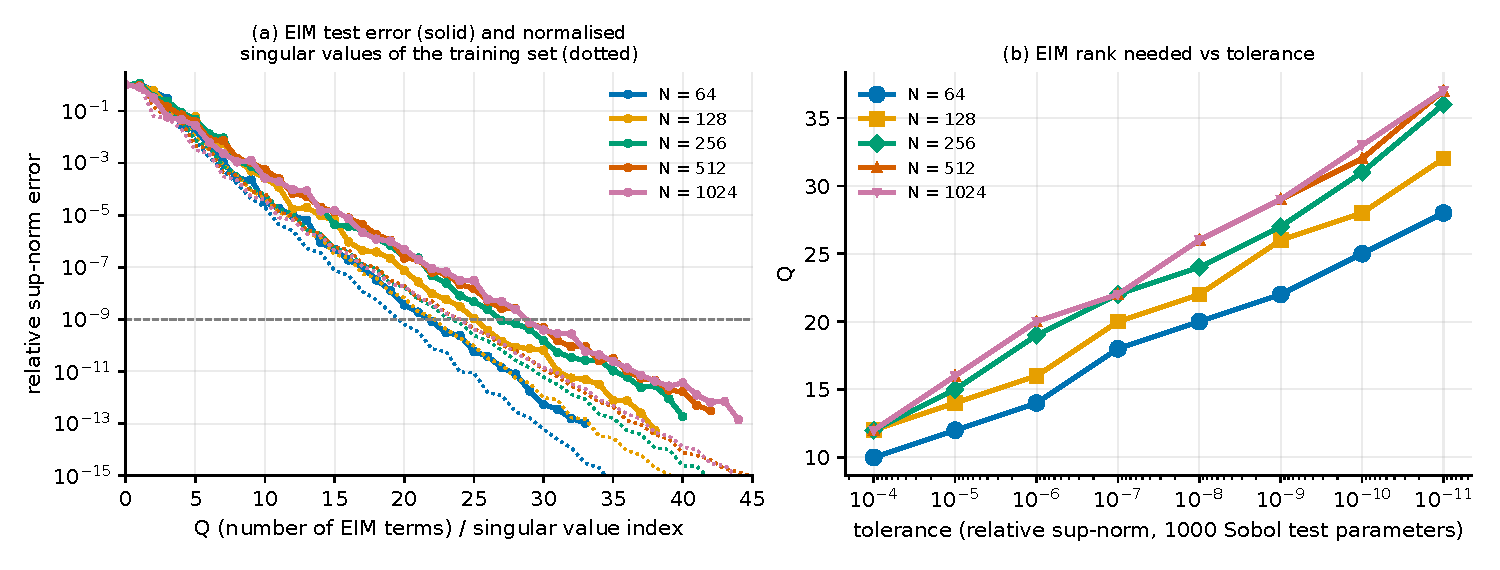
\includegraphics[width=0.8\linewidth]{F4_eim.pdf}
\caption{Empirical interpolation of the fractional symbol family.  (a) Relative sup-norm error on
$1000$ Sobol test parameters (solid) and normalised singular values of the $16^3$ training snapshots
(dotted), $N=64$--$1024$.  (b) Rank $Q$ needed for a given test tolerance; the curves for $N=512$ and
$N=1024$ coincide.  The operational $Q$ additionally satisfies the operator-norm check
(one extra term at $N=64$).}
\label{fig:eim}
\end{figure}
The error $\varepsilon_Q(\mu)$ is evaluated, not estimated: it is the sup-norm of the
interpolation error of the exact symbol at the query with the grid-to-continuum margin of
Lemma~\ref{lem:eim}.  Evaluated on the assembly grid it costs $O(LK)$ operations, which grows with
$N$; the implementation instead evaluates it on a fixed set of $161$ nodes (the graded grid of
Section~\ref{ssec:spectral}, coarsened) with the cell-wise derivative margin, which bounds the
continuous sup-norm and hence, by Remark~\ref{rem:compression}, the assembled operator difference,
at a cost of about $1.6$~ms independent of $N$ and at most $2.1$ times the value on the full grid.
Outside the training box of the interpolant the same evaluation remains rigorous and simply grows
(Section~\ref{ssec:ood}).
\begin{theorem}[Certificate with an affine surrogate operator]\label{thm:eim-cert}
Let the candidate trajectory be produced by any method (e.g.\ the reduced
system $V^\top A_Q(\mu)V$), and let $\rho_Q^{n+1/2}$ be its residual
evaluated with $A_Q$.  Then its residual with respect to the true assembled
system satisfies
\[
 \norm{\rr^{n+1/2}}_{S_I^{-1}}\ \le\ \norm{\rho_Q^{n+1/2}}_{S_I^{-1}}
 +\varepsilon_Q(\mu)\,\alpha_{\rm lb}^{-1/2}\,\norm{\overline{\bar\cc}_\theta^{\,n+1/2}}_2,
 \qquad \alpha_{\rm lb}=\smin(\mu),
\]
where $\bar\cc_\theta^n=Ez_\theta^n+b^n$ is the raw coefficient vector including the prescribed
entries (the surrogate operator also enters the lifting term of $f_I$), and
Theorem~\ref{thm:fully-discrete-certificate} holds with
\[
\eta^2=\beta_0^2+\dt\sum_n\bigl(\norm{\rho_Q}_{S^{-1}}+\varepsilon_Q\alpha_{\rm lb}^{-1/2}\norm{\overline{\bar\cc}_\theta}_2\bigr)^2.
\]
The same holds with $X_I$ in place of $S_I$ and $\min_\vartheta \sym{x}_\mu(\vartheta)\ (\ge \rf\,m_{\min})$ in place of $\alpha_{\rm lb}$.
\end{theorem}
\begin{proof}
$\rho=\rho_Q+E^\top(\bar A_h-\bar A_Q)\overline{\bar\cc}_\theta$ with the raw sections $\bar A_h,\bar A_Q$,
for which Lemma~\ref{lem:eim} gives the same $\varepsilon_Q$; bound the second term by
$\norm{(\bar A_h-\bar A_Q)\overline{\bar\cc}}_2\lambda_{\min}(S_I)^{-1/2}$ and use
Theorem~\ref{thm:spectral}.  This is exactly the allowance structure of
Remark~\ref{rem:arithmetic-scope}, with $d_n$ now explicit.
\end{proof}
The allowance is of size $\varepsilon_Q\norm{\bar\cc}_2/\sqrt{\alpha_{\rm lb}}$ per step, and for
accurate candidates it is the quantity that sets the EIM rank: with $\varepsilon_Q\approx10^{-9}\norm{\Ah}_2$,
$\norm{\Ah}_2\sim h^{-Y}$ and $\norm{\bar\cc}_2\sim \mathcal K\sqrt{N}\sqrt h$, its time-accumulated size at
$N=512$ with $Q=29$ is $6.8\times10^{-5}$ (median) to $4.3\times10^{-4}$ (maximum) in the $M_I$ norm on the
validation queries, comparable with the residual of a rank-$56$ reduced solution; its maximum drops to
$3.9\times10^{-6}$ with $Q=37$.  This dictates two design choices: the EIM tolerance is chosen as a
function of the target,
$\varepsilon_Q\norm{\bar\cc}_2\sqrt{T/\alpha_{\rm lb}}\le\varepsilon/10$, and the full-order
certificate should evaluate the residual with the exact operator $\Ah$ (two FFTs per step, no
allowance), reserving $A_Q$ for the reduced solve and for the $N$-independent online certificate.
\begin{remark}[Reduced online certificate]\label{rem:reduced-online}
With a fixed comparison norm $\bar X=\Tn{}{\bar{\sym{x}}}$, $\bar{\sym{x}}=\bar r\,\sym{m}+\bar\beta\,\sym{g}_1$,
chosen for a cell of parameter space such that $\bar r\le \rf$ and $\bar\beta\le\beta_\mu$ on the cell,
and the affine $A_Q$, the offline/online decomposition of the residual norm applies: the online cost of
$\eta^{\bar X}$ for a rank-$r$ candidate is $O(\varrho\,(Q+2)(2r+1))$ operations with $\varrho\le N_h$ retained rows
of the compressed $R$-factor, independent of $N_h$ once $\varrho$ saturates.  Since
$\bar{\sym{x}}\le\sym{x}_\mu\le\sym{s}_\mu$ on the cell, $\rho^\top S_I^{-1}\rho\le\rho^\top\bar X^{-1}\rho$ with no
further factor; the optional factor $(\inf_\vartheta\sym{s}_\mu/\bar{\sym{x}})^{-1}\le1$ of
Lemma~\ref{lem:toeplitz} tightens the bound at the cost of one symbol evaluation.  Because
$\sym{s}_\mu-\rf\,\sym{m}$ is proportional to $C$, $\beta_\mu=C\tilde\beta(G,M,Y)$, and since
$I_a(\xi)$ is decreasing in $a$ (the factor $e^{-ax}$), $\tilde\beta$ is nonincreasing in $G$ and in
$M$; the cells are therefore taken in $(C,Y,\min(G,M))$, not in $\rf$, the minimum over $C$ and over
$(G,M)$ is attained at the cell's corner $(C_{\min},G_{\max},M_{\max})$ exactly, and only the
one-dimensional minimum over $Y$ is taken on a grid with the safety factor $0.99$.
\end{remark}

\subsection{Candidates, initial target and training objective}
\label{ssec:target}\label{ssec:architectures}\label{ssec:exact-ic}\label{ssec:losses}\label{sec:data}
A candidate predicts coefficients in the fixed spline space, $(\mu,T,\psi,\tau)\mapsto
\cc_\theta(\tau;\mu,T,\psi)$ and $U_{\theta,h}=\sum_k c_{\theta,k}\phi_{h,k}$; its prescribed coefficients are overwritten at every time level before certification, which makes
it admissible in the same affine space as the reference, and its residuals use the assembled
operator of Section~\ref{ssec:assembly}.  The initial vector is the solver's specified target: the
raw mass projection $\bar M\bar\cc^0=\bar\bb^0$ with $\bar b_k^0=(\psi,\phi_{h,k})_{L^2(\Omega)}$,
followed by the imposition of the prescribed coefficients, with free part $\zz_h^0=E^\top\cc_h^0$; all
reference and training trajectories use it, and the initial discrepancy
$\beta_0=\|\zz_h^0-\zz_\theta^0\|_{M_I}$ is evaluated explicitly for every candidate (it vanishes
when the candidate embeds the target, $\cc_\theta(\tau)=\cc_h^0+\tau\mathcal N_\theta$, and is the
projection error for reduced trajectories).  The neural candidate of the production study is the
POD-NN of Section~\ref{ssec:pod-construction}; a DeepONet stress test is reported in
Section~\ref{sm:deeponet} of the supplementary materials.

The training objective combines the relative mass-weighted data loss
$\mathcal L_{\rm data}=(\cc_\theta-\cc_h)^\top\Mh(\cc_\theta-\cc_h)/(\cc_h^\top\Mh\cc_h+\epsilon)$,
the relative squared $L^2(\Omega)$ error of the homogeneous spline field with a small
$\epsilon>0$, and the residual regulariser
\begin{equation}
 \mathcal L_{\rm res}
 =\frac{1}{N_T}\sum_{n=0}^{N_T-1}
 (\rr_\theta^{n+1/2})^\top\Sh(\mu)^{-1}\rr_\theta^{n+1/2},
 \qquad \mathcal L=\mathcal L_{\rm data}+\lambda_R\mathcal L_{\rm res},
 \label{eq:residual-loss}
\end{equation}
with $\rr_\theta^{n+1/2}$ given by \eqref{eq:cn-residual}; on a uniform grid
$\etaSharp^2=T\mathcal L_{\rm res}$, so the regulariser controls the absolute mass error together
with the initial term, whereas the data loss is normalised.  The training set consists of 800
Sobol-sampled trajectories (seed 0) of the exact-assembly reference at the production resolution,
with a separate 30-query validation set (seed 999999) used for checkpoint selection and a
4000-trajectory set for the data-size study; Table~\ref{tab:training} in the supplementary materials
lists the optimiser, schedule, parameter counts and wall times.

\subsection{Mass-weighted POD trajectories}
\label{ssec:pod-construction}
With $M_I=LL^\top$ and the uncentred free snapshot matrix $Z$, define
$V=L^{-\top}U_r$, where $U_r$ contains the leading left singular vectors of
$L^\top Z$. Then $V^\top M_IV=I$ and the subspace minimises the aggregate
training-snapshot projection error in the mass norm. The 800 trajectories
supply 192,800 snapshots ($241$ time levels each). The reduced equations are
\begin{equation}
 \frac{\alpha^{n+1}-\alpha^n}{\dt}
 + (V^\top A_I V)\frac{\alpha^{n+1}+\alpha^n}{2}
 = V^\top f_I^{n+1/2},\qquad
 \alpha^0=V^\top M_I \zz_h^0.
 \label{eq:repaired-pod-cn}
\end{equation}

The reconstructed free candidate $V\alpha^n$ shares the prescribed boundary
coefficients. Its finite-rank initial discrepancy $\beta_0=\norm{(I-VV^\top M_I)\zz_h^0}_{M_I}$
is the projection error of the initial target and enters the same certificate as the neural
candidate.

\paragraph{POD--Galerkin with the affine operator.}
With $A_Q$ in place of $A_I$ the reduced operator is
\[
V^\top A_Q(\mu)V=-(\rf-\omega_S)\,V^\top D_IV+\lambda_0 I-C\Gamma(-Y)h^{-Y}\sum_q\ell_q(\nu)\,V^\top T_qV,
\]
a combination of $Q+2$ precomputed $r\times r$ matrices with scalar coefficients, and the
reduced forcing is affine in the same scalars and in the two lifting values $b_L(\tau_n)$, through
the precomputed vectors $V^\top M_I e_{\rm bd}$, $V^\top T_q e_{\rm bd}$.  The online solve therefore
costs $O(Qr^2+N_Tr^2)$ operations and never touches the full space.  The candidate is certified
either at full order, by Theorem~\ref{thm:eim-cert} with $\eta^X$ or $\eta^S$ and the allowance
term, or online as follows.

\paragraph{Reduced online certificate.}
Fix a comparison matrix $\bar X=r_{\min}M_I+\bar\beta\,h^2R^{(1)}_I$ per cell of a coarse
partition of the $(C,Y,\min(G,M))$ range, with $\bar\beta=0.99\min_{\rm cell}\beta_\mu$ evaluated on
a grid of the cell (Remark~\ref{rem:reduced-online}).  Then $\rho^\top\bar X^{-1}\rho$ is a quadratic form in the
$Q+2$ scalar coefficients and the reduced states, whose $(Q+2)^2$ Gram blocks
$R_q^\top\bar X^{-1}R_{q'}$, $R_q\in\{M_IV,\,T_qV,\,D_IV,\,\text{forcing directions}\}$, are
computed offline by banded solves.  Online, $\eta^{\bar X}$ is an upper bound for the exact dual norm
without any further factor (Remark~\ref{rem:reduced-online}); the symbol quantities that accompany it, $\varepsilon_Q(\mu)$ and
the optional tightening factor, are evaluated on an $N$-independent graded grid with derivative
margins.  For accurate candidates the residual is $10^{-8}$ of the terms it is assembled from, a
regime in which the Gram-tensor form of the offline/online decomposition loses all digits; the
implementation therefore uses the numerically stable $R$-factor form
\cite{CasenaveErnLelievre2014,BuhrEngwerOhlbergerRave2014}, compressed offline by a singular value
decomposition with rigorous terms for the discarded part and for rounding.  The online cost is then
$O(\varrho\,(Q+2)(2r+1))$ with $\varrho$ retained rows ($185$--$1022$ for $r=8$--$128$ at $N=1024$;
$\varrho$ saturates below $N_h$, which is what makes the cost independent of $N$), the online
value agrees with the full-order $\rho^\top\bar X^{-1}\rho$ to $2\times10^{-10}$ for POD--Galerkin
candidates (the double-precision floor, confirmed in extended precision), and the compressed bound
exceeds the uncompressed one by at most $5\times10^{-4}$ relative.  The cell norm is within a
factor $1.87$ (median) of the query's own $X_I$ and about $4$ of $\eta^S$
(Table~\ref{tab:pod-ranks}).  On an idle core the complete online certificate takes
$2.9$--$8.3$~ms for $r=8$--$128$ ($Q=36$; Figure~\ref{fig:online-time}), of which $2.7$~ms are
rank-independent, and the offline tensors occupy $9$--$688$~MB for the 18 cells.

\paragraph{POD-NN.}
The neural reduced candidate maps $(\mu,T)$ to the $r\times N_T$ matrix of POD coefficients
$\alpha^1,\dots,\alpha^{N_T}$ by a multilayer perceptron, with $\alpha^0=V^\top M_I\zz_h^0$ fixed
so that $\beta_0$ is again the projection error only
\cite{HesthavenUbbiali2018}.  Its training objective is the least-squares loss in the reduced
coordinates (the mass-weighted loss $\mathcal L_{\rm data}$, since $V^\top M_IV=I$) plus
$\lambda_R$ times the reduced online certificate $\eta^{\bar X}_{\rm aug}$ of the previous paragraph
(not squared), which is a differentiable function of the network output and costs nothing per
sample; it plays the role of the residual regulariser \eqref{eq:residual-loss}, with the exact dual
norm replaced by a rigorous majorant.  The network is evaluated in double precision: single-precision rounding of the
predicted coefficients alone produces residuals whose certified bound is of the order $10^{-3}$ at
$N=512$, i.e.\ the tolerance itself.  The standard output has $r\times N_T=11\,520$ coefficients ($3.09$~M parameters, of which $2.96$~M in
the output layer).  A second variant predicts the coefficients of a temporal POD of the reduced
trajectories, $r\times r_t$ with $r_t=23$ modes chosen so that the temporal projection error is
below $\varepsilon_N/10$ ($0.42$~M parameters); it removes the time-difference noise that the
residual penalises by construction.  Both are trained with $\lambda_R\in\{0,10^{-2},10^{-1},1\}$ on
800 and 4000 trajectories (Table~\ref{tab:training}).

\subsection{Cost model}
\label{ssec:cost}
Per query and time step, the direct solve costs ${\rm it}_B$ preconditioned GMRES iterations, each
with two FFTs of length $2N_h$ (${\rm it}_B=5$--$9$, Table~\ref{tab:pcg-v9}); the certificate $\eta^X$
costs one residual evaluation (two FFTs) and one banded solve; the reduced solve and the reduced
certificate cost $O(r^2)$ and $O(r(Q+2))$ operations, after $O((Q+2)r^2)$ and
$O(\varrho\,(Q+2)(2r+1))$ operations per query with $\varrho\le N_h$ retained rows.  Section~\ref{sm:cost}
of the supplementary materials gives the operation counts and the measured constants.  Two conclusions are
independent of the implementation.  First, at full order the certificate $\eta^X$ costs one
residual evaluation per step, a small fraction (about $1/{\rm it}_B$) of the direct solve, for
every candidate.  Second, the reduced solve and certificate do not
involve $N_h$ once the offline compression has fixed $\varrho$: a certified reduced query costs
$O(\varrho\,Q\,r)$ operations at any resolution, with the rigorous link to the full-order problem
supplied by Theorem~\ref{thm:eim-cert} and Lemma~\ref{lem:toeplitz}.

\section{Numerical evaluation}
\label{sec:numerics}
\subsection{Experimental design}
\label{ssec:design}\label{tab:populations}
All studies use the exact assembly of Section~\ref{ssec:assembly} ($K=100$), quadratic splines,
the box of \eqref{eq:numerical-box} and the free system.  The verification studies use 60
Crank--Nicolson steps at several $N$ on 32 box vertices and 256 Sobol points (288 queries) and on 48
exact-dynamics queries with perturbed initial vectors; the production studies from
Section~\ref{ssec:calibration} on use the configuration fixed there, $N=1024$, $N_T=240$,
$\varepsilon_N=1.18\times10^{-3}$, and report every verdict at the sweep
$\varepsilon_N\times\{0.1,0.3,1,3,10\}$.  Their populations are the 30 price-diagnostic queries and
two box corners of the calibration (five spots $0.8\mathcal K,\dots,1.2\mathcal K$), the 800 and 4000
Sobol training trajectories (seed 0) with a 30-query validation set (seed 999999) on which the
reduced models and candidates are studied, 120 Sobol benchmark queries, $10^4$ Sobol queries for the
multi-query study, and 200 Sobol queries outside the box plus 64 extended vertices for the
out-of-distribution study.  Statistics over spots first take the maximum within each query, and
bootstrap intervals resample queries.
\subsection{Verification of the assembly, the bounds and the solvers}
\label{ssec:verification}\label{ssec:e0-assembly}\label{ssec:e0-spectral}\label{ssec:e0-riesz}\label{ssec:e0-initial}
The verification studies, reported in full in Section~\ref{sm:verification} of the supplementary
materials, confirm every ingredient of the certificate.  The assembled free matrix agrees with the
exact Galerkin matrix, computed independently at 40 digits, to $10^{-8}$ in operator norm at $K=100$,
the truncation error decreases like $K^{-(2p-Y-1)}$ as Lemma~\ref{lem:tail} predicts, and the bound
$\varepsilon_K$ is within a factor $1.1$--$3.7$ of the observed error at $K=100$
(Table~\ref{tab:assembly-v9}).  The bound of Theorem~\ref{thm:spectral} and the two-sided comparison
\eqref{eq:comparison} hold at all $289\times3$ tested (query, $N$) pairs; the a-priori factor
$\sqrt{\Thmu}$ grows like $(\min(G,M)h)^{(Y-2)/2}$ (median $2.05$ at $N=1024$), while the observed
ratio $\eta^X/\eta^S$ on candidates stays below two at the production resolution
(Figures~\ref{fig:spectral-bound} and~\ref{fig:theta}).  Circulant-preconditioned conjugate
gradients solve the Riesz systems in $8$--$12$ iterations for $N=64$--$4096$, and the GMRES solve of
$B_+$ needs $5$--$9$ iterations per step on average (Table~\ref{tab:pcg-v9}).  On exact dynamics with
perturbed initial vectors both augmented bounds hold with effectivity $1.00\pm10^{-6}$, and for
$Y\in\{0.5,0.8,0.95\}$ the bound $\alpha_{\rm lb}=\rf$ is positive and the certificate holds with
effectivity one, so the discrete framework covers the finite-variation regime without change.
\subsection{Resolution and tolerance calibration}
\label{ssec:calibration}
The production resolution is the smallest $N$ at which the discrete put price is within one cent
of the COS reference \cite{FangOosterlee2008} (8192 modes, range parameter 30; agreement with
Carr--Madan to $2.6\times10^{-12}$ on the checked rows) at the five spots $0.8\mathcal K,\dots,1.2\mathcal K$, over the
30 price-diagnostic queries and the two short-maturity, weakly diffusive box corners
($C=0.05$, $Y=1.1$, $T=0.1$) that had price gaps above two dollars at $N=64$.
Table~\ref{tab:budget} gives the maxima.  The 30 queries alone would pass at $N=512$ ($0.11$ cent),
the corners do not ($2.4$ and $3.2$ cent); at $N=1024$ all are at most $0.235$ cent with 240 steps,
whereas 60 steps give $4.6$ cent on the 30 queries at that resolution.  With the spot factor
$\max_s\beta_I(x_s)=8.44$ of \eqref{eq:gamma-infty}, one cent corresponds to the trajectory
tolerance $\varepsilon_N=1.18\times10^{-3}$; this configuration is fixed once and not changed by
any later experiment.  A tenth of a cent ($\varepsilon_N/10$) is reported as a certificate
tolerance only, since the discretisation error at $N=1024$ is $0.235$ cent.
\begin{table}[!htbp]
\centering\small
\caption{Resolution and tolerance calibration: maximum price error $\max|V_h(T,S)-V_{\mathrm{COS}}|$ over the 30 price-diagnostic queries and the two box corners, spots $S\in\{0.8,\dots,1.2\}\mathcal K$; COS with 8192 modes, range parameter 30. $\varepsilon_N=\tau_\$/\max_s\beta_I(x_s)$ with $\tau_\$=1$ cent.}
\label{tab:budget}
\begin{tabular}{rrrrrrr}
\toprule
$N$ & $N_T$ & 30 queries & corner A & corner B & $\max_s\beta_I$ & $\varepsilon_N$\\
\midrule
128 & 60 & $0.0361$ & $0.703$ & $0.783$ & $3.103$ & $3.22\times10^{-3}$\\
128 & 240 & $0.0361$ & $0.703$ & $0.783$ & $3.103$ & $3.22\times10^{-3}$\\
256 & 60 & $2.82\times10^{-3}$ & $0.172$ & $0.203$ & $4.396$ & $2.28\times10^{-3}$\\
256 & 240 & $2.80\times10^{-3}$ & $0.172$ & $0.203$ & $4.396$ & $2.28\times10^{-3}$\\
512 & 60 & $6.17\times10^{-3}$ & $0.0236$ & $0.0316$ & $6.073$ & $1.65\times10^{-3}$\\
512 & 240 & $1.12\times10^{-3}$ & $0.0236$ & $0.0316$ & $6.073$ & $1.65\times10^{-3}$\\
1024 & 60 & $0.0464$ & $1.36\times10^{-3}$ & $2.36\times10^{-3}$ & $8.441$ & $1.18\times10^{-3}$\\
1024 & 240 & $1.59\times10^{-3}$ & $1.35\times10^{-3}$ & $2.35\times10^{-3}$ & $8.441$ & $1.18\times10^{-3}$\\
\bottomrule
\end{tabular}
\end{table}

\subsection{Reduced model and neural candidates}
\label{ssec:e1}\label{ssec:pod-results}
Table~\ref{tab:pod-ranks} and Figure~\ref{fig:acceptance} report the POD--Galerkin candidates on
the validation set at the production configuration.  The mass-weighted basis from 800 trajectories
reaches a median error of $3.1\times10^{-4}$ at $r=48$ and $1.7\times10^{-5}$ at $r=64$, and 800
trajectories already capture the solution manifold: five times more training data leaves the
singular values within $10\%$ up to $r=48$ and within a factor $1.5$ up to $r=128$.  The
exact certificate has effectivity $9$--$15$ for $16\le r\le80$ ($6.8$ at $r=8$), consistent with Theorem~\ref{thm:efficiency}
(efficiency holds in the energy norm, which weights the high-frequency part of the error far more
than the mass norm in which the error is measured); the banded certificate is a further factor
$\approx2$ above it, as predicted by $\sqrt{\Thmu}$, and the reduced online certificate a further
factor $\approx2$, the cell factor.  Acceptance at one cent therefore starts at $r=56$ under the
exact certificate (28 of 30), at $r=62$--$64$ under all three, and is complete at $r\ge80$.  The
three-stage rule settles every query at $r\le48$ by cheap rejection and every query at $r\ge80$ by
reduced acceptance; the full-order stages are needed only in the band $r=56$--$64$.  No false
accept occurs under any certificate at any tolerance.  At $r\ge96$ the true error ($4\times10^{-8}$)
falls below the floor set by the EIM allowance at $Q=36$, which raises the reduced effectivity to
$230$--$420$ while every query is still accepted.
\begin{table}[!htbp]
\centering\small
\caption{POD--Galerkin candidates on the 30 validation queries at the production configuration ($N=1024$, $N_T=240$, $Q$ matched to $\varepsilon$): median maximum-in-time mass-norm error against the direct solution, median effectivity (bound/error) of the three certificates, queries accepted at $\varepsilon_N=1.18\times10^{-3}$ under each certificate, and the stage at which the three-stage rule of Proposition~\ref{prop:threestage} settles the query (reduced accept / cheap reject / banded accept / exact accept / exact reject). Basis from 800 training trajectories; the 4000-trajectory basis gives the same picture (Section~\ref{ssec:e1}). No false accepts occur under any certificate at any tolerance of the sweep.}
\label{tab:pod-ranks}
\resizebox{\textwidth}{!}{%
\begin{tabular}{rrrrrrr}
\toprule
$r$ & error & eff.\ $\eta^S$ & eff.\ $\eta^X$ & eff.\ $\eta^{\bar X}$ & accepted $\bar X$/$X$/$S$ & three-stage\\
\midrule
8 & 1.19 & 6.8 & 10.8 & 24 & 0/0/0 & 0/30/0/0/0\\
16 & 0.139 & 14.9 & 25.2 & 50 & 0/0/0 & 0/30/0/0/0\\
24 & 0.0298 & 13.9 & 25.2 & 52 & 0/0/0 & 0/30/0/0/0\\
32 & $7.1\times10^{-3}$ & 13.3 & 23.2 & 48 & 0/0/0 & 0/30/0/0/0\\
40 & $1.3\times10^{-3}$ & 13.2 & 24.1 & 47 & 0/0/0 & 0/30/0/0/0\\
48 & $3.1\times10^{-4}$ & 11.7 & 21.6 & 49 & 0/0/0 & 0/30/0/0/0\\
56 & $6.0\times10^{-5}$ & 11.5 & 21.5 & 47 & 0/9/28 & 0/2/9/19/0\\
62 & $1.9\times10^{-5}$ & 11.3 & 22.0 & 50 & 24/30/30 & 24/0/6/0/0\\
64 & $1.7\times10^{-5}$ & 10.5 & 20.0 & 42 & 26/30/30 & 26/0/4/0/0\\
80 & $6.6\times10^{-7}$ & 9.5 & 19.3 & 47 & 30/30/30 & 30/0/0/0/0\\
96 & $3.6\times10^{-8}$ & 9.1 & 16.8 & 231 & 30/30/30 & 30/0/0/0/0\\
128 & $9.9\times10^{-9}$ & 4.3 & 5.3 & 417 & 30/30/30 & 30/0/0/0/0\\
\bottomrule
\end{tabular}}
\end{table}

\begin{figure}[!htbp]
\centering
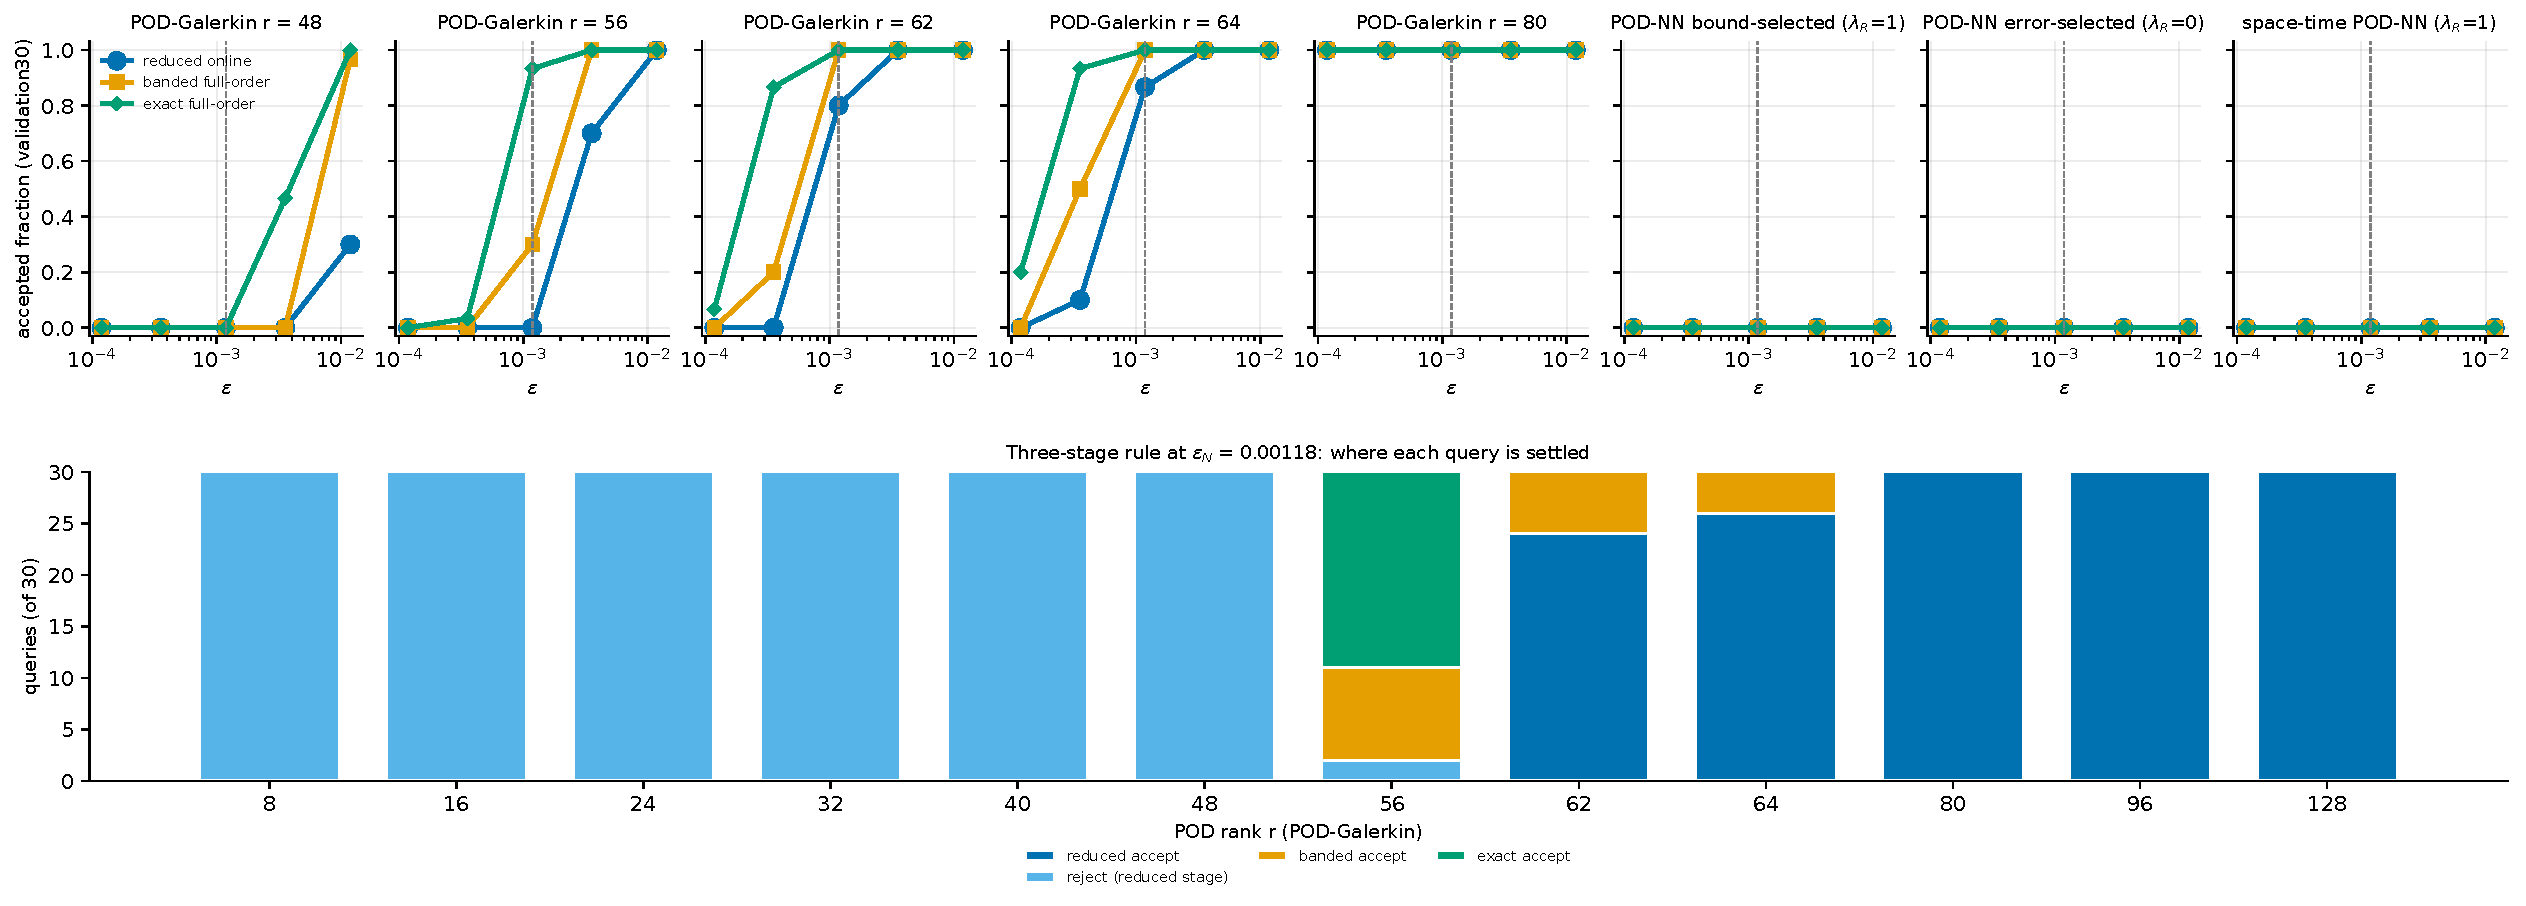
\includegraphics[width=0.78\linewidth]{F5a_acceptance.pdf}
\caption{Top: accepted fraction of the 30 validation queries as a function of the tolerance
$\varepsilon$ (dashed line: $\varepsilon_N$) for POD--Galerkin candidates of rank $48$--$80$ and the
two best POD-NN checkpoints, under the reduced online, banded full-order and exact full-order
certificates.  Bottom: the stage at which the three-stage rule of Proposition~\ref{prop:threestage}
settles each query at $\varepsilon_N$, per rank.}
\label{fig:acceptance}
\end{figure}

The neural candidates are reported in Table~\ref{tab:podnn} of the supplementary materials, and
the certificate gives a precise account of them.  At $\varepsilon_N$ (and at $10^{-3}$) it rejects
every neural prediction: the best standard-output network ($4000$ trajectories, $\lambda_R=1$) has a
median true error of $0.46$ and a median exact bound of $1.26$, about $10^3\varepsilon_N$; the
space--time variant improves both by an order of magnitude (errors $0.014$--$0.016$ and bounds
$0.054$--$0.058$ over three seeds, $46$--$49\,\varepsilon_N$).  Three observations explain these
numbers.  With $\lambda_R=0$ the network fits the coefficients best (error $0.08$) but its trajectory
is noisy in time, and the residual, which contains the time difference divided by $\dt$, gives a
bound of $12$ (effectivity $150$); with $\lambda_R>0$ the bound drops by a factor ten while the error
rises by a factor five, so the residual term buys temporal smoothness with accuracy, and selecting
checkpoints by the rigorous bound picks the smoother, less accurate network (bound $1.26$, error
$0.46$, against bound $12.2$, error $0.082$ when selecting by the true error, which requires the
reference).  The space--time representation removes the temporal noise by construction and
improves both measures.  Finally, the projection of the reference trajectories onto the same basis,
certified at $3.2\times10^{-3}$, shows that the basis is adequate, so the remaining gap lies in the
coefficient map; the selected epochs ($1890$--$2000$ of $2000$) show that the bound was still
decreasing at the end of training, and the space--time result indicates that the representation,
rather than the training length, is the lever for closing a gap of $46$--$1000$.  Every neural query is
settled by the cheap rejection of the first stage, in milliseconds and with no false accept.  Figure~\ref{fig:online-time} shows the online cost of the
reduced model on the validation queries: the reduced solve takes $0.7$--$2.0$~ms and the reduced
certificate $2.9$--$8.3$~ms for $r=8$--$128$; the three-stage total at $\varepsilon_N$ equals the
reduced certificate wherever the first stage decides ($r\le48$ by cheap rejection, $r\ge62$ by
acceptance) and rises to $154$~ms only at $r=56$, where the full-order stages are needed.
\subsection{Matched benchmark and cost under refinement}
\label{ssec:benchmark}\label{ssec:scaling-results}
Table~\ref{tab:benchmark} and Figure~\ref{fig:benchmark} report the 120 benchmark queries at the
production configuration.  The baseline is the \emph{uncertified} circulant-preconditioned GMRES
solve of Section~\ref{ssec:e0-riesz} ($259$~ms with reusable setup, $337$~ms cold); every ratio is a
geometric mean over queries with a $95\%$ query-bootstrap interval, and the certificate cost of the
direct solve is shown separately.  Three results.

First, the full-order certificate is cheap: the banded certificate $\eta^X$ with the exact
operator costs $6.0\%$ of the solve ($7.2\%$ including the per-query spectral data in the fast
online mode of Section~\ref{ssec:spectral}), so a certified direct solve takes $1.06$ times an
uncertified one, and this fraction stays at $4.5$--$5.6\%$ from $N=64$ to $N=4096$
(Figure~\ref{fig:benchmark}, right), as the cost model of Section~\ref{ssec:cost} predicts
(Table~\ref{tab:cost}).  The fast mode (a coarse graded grid of $1012$ nodes with ten aliases and a
rigorous $\sin^{2p}$-weighted tail) reproduces $\beta_\mu$ and $\Thmu$ to $0.2\%$ and changes
$\eta^X$ by $0.002\%$, whereas the fine verification grid of Section~\ref{ssec:e0-spectral} costs
$478$~ms and would make the certified solve $2.92$ times the uncertified one.

Second, the certified reduced model is an order of magnitude faster than the direct solve
whenever the three-stage rule stops at the reduced stage: POD--Galerkin with $r=80$ takes
$0.032$ of the direct time ($8.3$~ms) at every tolerance of the sweep, with all 120 queries accepted
at the $N$-independent stage; with $r=64$ it takes $0.041$ at $\varepsilon_N$ (102 reduced and 18
banded accepts), $0.026$ at $3\varepsilon_N$, and $0.55$ at $0.3\varepsilon_N$, where most queries
need a full-order stage and four need correction (without reusable setup the ratio rises to $0.30$
because the query-independent initial projection, $90$~ms, is rebuilt inside the timer).
Third, the rule caps the cost of an inadequate candidate: the neural candidate is rejected at the
reduced stage in a few milliseconds per query and then corrected by a full-order march warm-started
from the candidate and re-certified, for a total of $1.07$ times the direct solve at every
tolerance, so every query still returns a certified price.  No false accept occurs for any method
or tolerance.
\begin{figure}[!t]
\centering
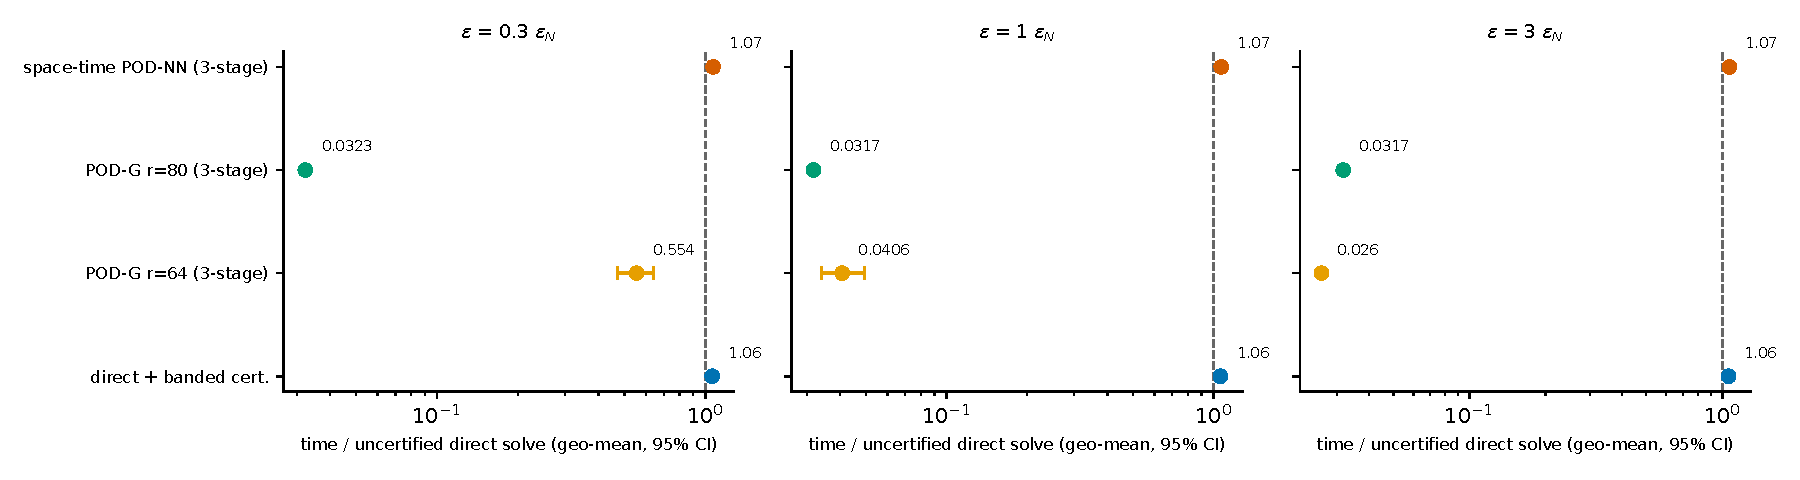
\includegraphics[width=0.76\linewidth]{F6a_benchmark.pdf}\\[2mm]
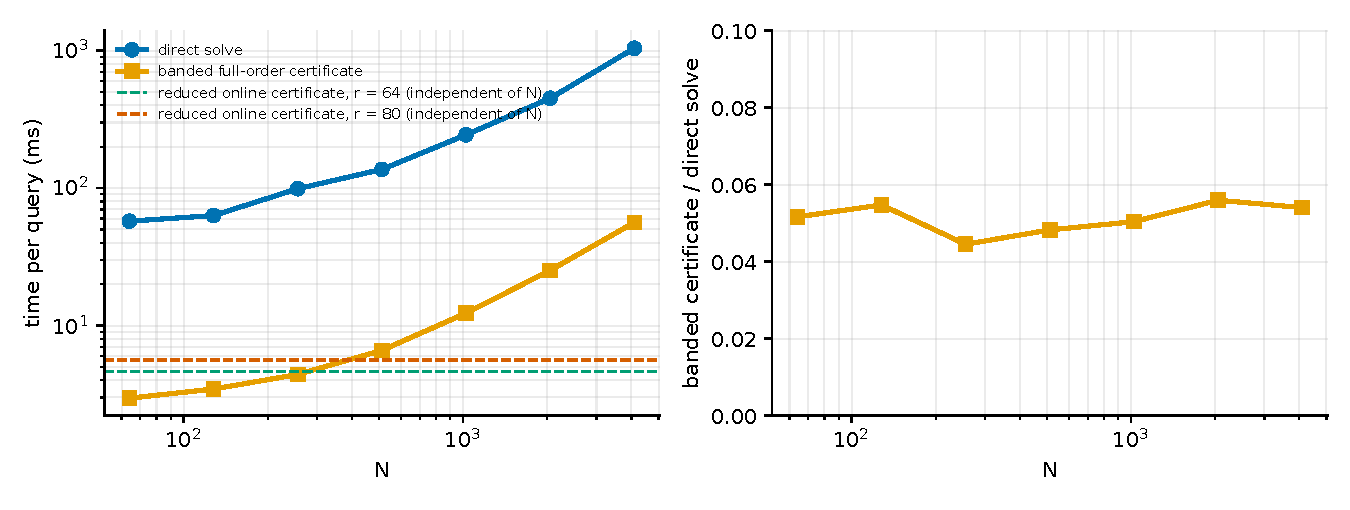
\includegraphics[width=0.76\linewidth]{F6b_refinement.pdf}
\caption{Top: time ratio to the uncertified direct solve on the 120 benchmark queries at
$\varepsilon=0.3\varepsilon_N$, $\varepsilon_N$, $3\varepsilon_N$ (geometric means, $95\%$
query-bootstrap intervals, reusable setup).  Bottom left: direct solve and banded full-order
certificate per query as functions of $N$ (20 benchmark queries, $N_T=240$), with the reduced
online certificate at $r=64$ and $80$, which does not depend on $N$.  Bottom right: the certificate
as a fraction of the solve, $4.5$--$5.6\%$ for $N=64$--$4096$.}
\label{fig:benchmark}
\end{figure}
\begin{table}[!htbp]
\centering\small
\caption{Matched benchmark on the 120 benchmark queries at the production configuration (one thread, idle machine, reusable setup, five repetitions): geometric-mean time ratio to the uncertified direct solve with 95\% query-bootstrap interval, three-stage outcome (reduced accept / cheap reject / banded or exact accept / corrected), and false accepts.  The direct solve takes $259$~ms; the certificate proper is $6.0\%$ of it and $7.2\%$ with the per-query spectral data.}
\label{tab:benchmark}
\begin{tabular}{llrcr}
\toprule
$\varepsilon$ & method & time ratio (CI) & outcome & f.a.\\
\midrule
-- & direct $+$ banded certificate & 1.06 (1.06--1.06) & cert.\ fraction 0.07 & --\\
$0.3\varepsilon_N$ & POD--Galerkin $r=64$ & 0.554 (0.47--0.642) & 8/4/108/4 & 0\\
$0.3\varepsilon_N$ & POD--Galerkin $r=80$ & 0.0323 (0.032--0.0326) & 120/0/0/0 & 0\\
$0.3\varepsilon_N$ & space--time POD-NN & 1.07 (1.06--1.07) & 0/120/0/120 & 0\\
$1\varepsilon_N$ & POD--Galerkin $r=64$ & 0.0406 (0.034--0.0494) & 102/0/18/0 & 0\\
$1\varepsilon_N$ & POD--Galerkin $r=80$ & 0.0317 (0.0314--0.032) & 120/0/0/0 & 0\\
$1\varepsilon_N$ & space--time POD-NN & 1.07 (1.06--1.07) & 0/120/0/120 & 0\\
$3\varepsilon_N$ & POD--Galerkin $r=64$ & 0.026 (0.0257--0.0262) & 120/0/0/0 & 0\\
$3\varepsilon_N$ & POD--Galerkin $r=80$ & 0.0317 (0.0313--0.032) & 120/0/0/0 & 0\\
$3\varepsilon_N$ & space--time POD-NN & 1.07 (1.06--1.07) & 0/120/0/120 & 0\\
\bottomrule
\end{tabular}
\end{table}


\subsection{Out-of-distribution detection}
\label{ssec:ood}
The certificate makes no assumption about where a query lies, so the natural test is to leave the
box.  Table~\ref{tab:ood} reports 264 queries outside the box \eqref{eq:numerical-box}
(200 Sobol points in the shells $C\in[1,2]$, $Y\in[0.9,1.1)\cup(1.8,1.95]$, $G\in[0.5,1)$,
$M\in[9,15]$, excluding $|Y-1|<0.02$ where $\Gamma(-Y)$ is singular, and the 64 vertices of the
extended box).  Every query is certifiable: $\alpha_{\rm lb}=\rf-\varepsilon_K>0$ and the Toeplitz
aliasing stays below $10^{-15}$ even for $G<1$.  Outside the cells of Section~\ref{ssec:eim} the
three-stage rule starts at the banded stage with the query's own $X_I$, and the EIM error
$\varepsilon_Q$, evaluated at the query, grows by two orders of magnitude (median $2\times10^{-7}$
against $1.7\times10^{-9}$ inside the box) because the interpolant extrapolates in $Y$ and $G$; the
certificate accounts for this growth rigorously through the allowance.

Three facts follow.  There is no false accept for any candidate under any certificate at any
tolerance of the sweep, as Theorem~\ref{thm:fully-discrete-certificate} guarantees.  The reduced
model remains accurate on most of the extended domain, and the certificate recognises it:
POD--Galerkin with $r=80$ is within one cent on 210 of the 264 queries, and the certificate accepts
193 of them (92\%); the other 17 are conservative rejections (median effectivity $6.3$), concentrated
in the shells $Y>1.8$ and $G<1$, which are also the shells of largest $\varepsilon_Q$.  A detector that
rejects everything outside the training box has the same recall as the certificate but discards all
210 working queries (precision $0.20$ against $0.76$); seed-ensemble disagreement, the usual heuristic
for neural candidates, has no working query to score here, since every space--time POD-NN error
exceeds $\varepsilon_N$ in and out of the box.  In Figure~\ref{fig:ood} every point lies above the
diagonal.
\begin{table}[!htbp]
\centering\small
\caption{Out-of-distribution study: 264 queries outside the parameter box (200 Sobol points in the
shells $C\in[1,2]$, $Y\in[0.9,1.1)\cup(1.8,1.95]$, $G\in[0.5,1)$, $M\in[9,15]$, and 64 vertices of the
extended box) at the production configuration.  Top: queries on which the candidate's true error
is below $\varepsilon_N$ (``works''), queries the exact certificate accepts (``certified''), and
precision of two rules as detectors of ``true error $>\varepsilon_N$'': the certificate (recall 1 by
theorem) and the naive rule that rejects every query outside the training box (recall 1, but it
discards every working query).  Bottom: POD--Galerkin $r=80$ by shell (a query leaving the box in
several coordinates counts in each), with the median true error and the median EIM error
$\varepsilon_Q$ (inside the box: $1.7\times10^{-9}$).}
\label{tab:ood}
\begin{tabular}{lrrrr}
\toprule
candidate & works & certified & precision (certificate) & precision (naive rule)\\
\midrule
POD--Galerkin $r=64$ & 196 & 181 & 0.82 & 0.26\\
POD--Galerkin $r=80$ & 210 & 193 & 0.76 & 0.20\\
space--time POD-NN & 0 & 0 & -- & --\\
\bottomrule
\end{tabular}
\par\smallskip
\begin{tabular}{lrrrrr}
\toprule
shell ($r=80$) & queries & works & certified & median error & median $\varepsilon_Q$\\
\midrule
$C>1$ & 122 & 104 & 95 & $3.7\times10^{-6}$ & $5.3\times10^{-8}$\\
$Y<1.1$ & 39 & 36 & 31 & $6.1\times10^{-6}$ & $1.4\times10^{-8}$\\
$Y>1.8$ & 36 & 18 & 15 & $2.8\times10^{-3}$ & $6.1\times10^{-7}$\\
$G<1$ & 27 & 21 & 13 & $3.9\times10^{-4}$ & $3.1\times10^{-6}$\\
$M>9$ & 111 & 101 & 94 & $8.6\times10^{-6}$ & $2.5\times10^{-7}$\\
vertices & 64 & 34 & 31 & $2.0\times10^{-4}$ & $4.3\times10^{-6}$\\
\bottomrule
\end{tabular}
\end{table}

\begin{figure}[!htbp]
\centering
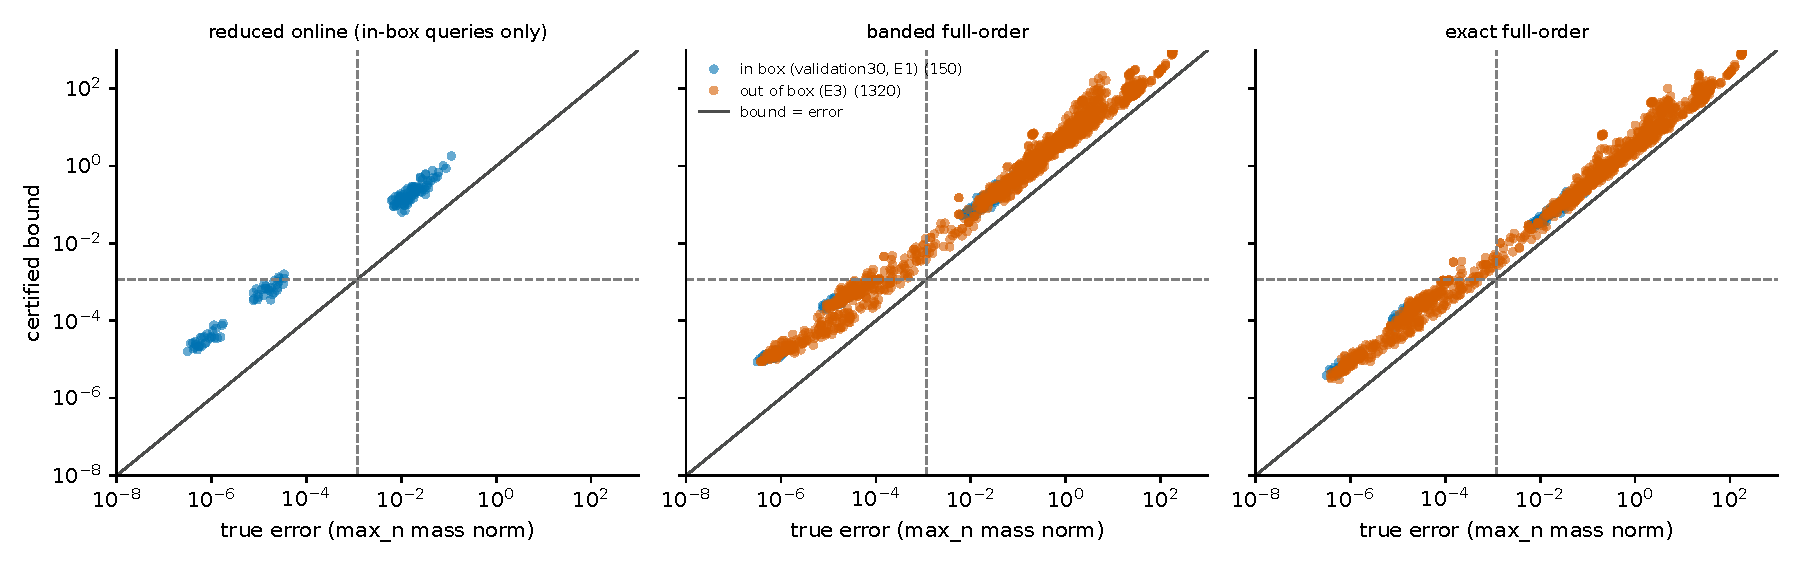
\includegraphics[width=0.72\linewidth]{F7_ood.pdf}
\caption{Certified bound against true error for the 264 out-of-box queries and the 30 validation
queries (POD--Galerkin $r=64$ and $80$, space--time POD-NN), under the three certificates; the lines
mark $\varepsilon_N$ and bound $=$ error.}
\label{fig:ood}
\end{figure}
\subsection{Multi-query cost and amortisation}
\label{ssec:multiquery}
Figure~\ref{fig:amortisation} reports $10^4$ Sobol queries at $\varepsilon_N$ on one core, with
every method's offline cost as the intercept.  The direct solve averages $260$~ms per query.
Certified POD--Galerkin with $r=80$ averages $9.0$~ms: $99.77\%$ of the queries are settled at the
reduced stage, $0.14\%$ at the banded stage, $0.02\%$ at the exact stage, and $0.07\%$ are rejected
and corrected; with $r=64$ the mean is $21.2$~ms (median $7.2$~ms; $89.7\%$ reduced, $9.8\%$ banded,
$0.35\%$ corrected).  The offline cost of the reduced model is about $1530$~s: reference
trajectories $208$~s, POD $797$~s, EIM $65$~s, cell constants $425$~s, offline tensors $39$~s
(single-thread equivalents; the POD used four BLAS threads).  The fitted totals
$T(Q)=1533\,\mathrm s+9.0\,\mathrm{ms}\cdot Q$ ($r=80$) and $1533\,\mathrm s+21.2\,\mathrm{ms}\cdot Q$
($r=64$) break even with $260\,\mathrm{ms}\cdot Q$ after about $6100$ and $6400$ queries.  The
space--time POD-NN never breaks even: its online cost exceeds the direct solve ($282$~ms, since
every query is corrected), and its offline cost ($2.7\times10^4$~s) is dominated by training.
This experiment measures verdicts and times; reliability is verified on the queries with reference
solutions in Sections~\ref{ssec:e1}--\ref{ssec:ood}.
\begin{figure}[!htbp]
\centering
\begin{minipage}[t]{0.49\linewidth}\centering
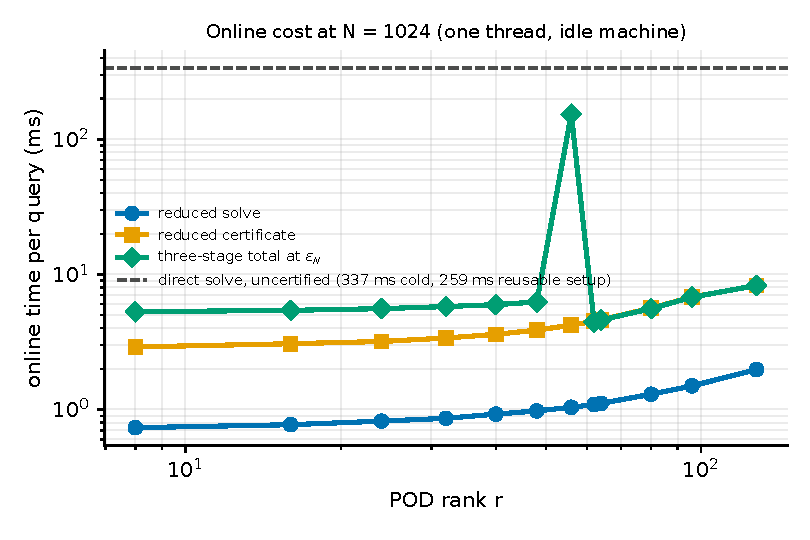
\includegraphics[width=\linewidth]{F5c_online_time.pdf}
\caption{Online time per query of the reduced model at the production configuration (one thread,
idle machine): reduced solve, reduced online certificate, and the three-stage total at
$\varepsilon_N$, against the uncertified direct solve (dashed: cold-start and reusable-setup medians of the
benchmark of Section~\ref{ssec:benchmark}).}
\label{fig:online-time}
\end{minipage}\hfill
\begin{minipage}[t]{0.49\linewidth}\centering
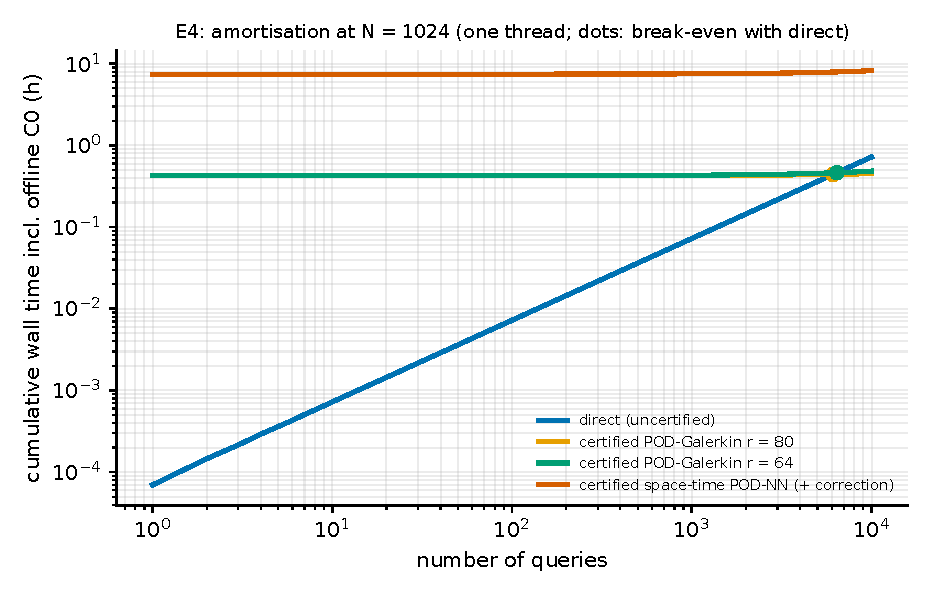
\includegraphics[width=\linewidth]{F8_amortisation.pdf}
\caption{Cumulative wall time, offline cost included, against the number of queries at the
production configuration (one thread); dots mark the break-even with the uncertified direct
solver.}
\label{fig:amortisation}
\end{minipage}
\end{figure}
\subsection{Reproducibility}
\label{ssec:archive}
All computations use the package \texttt{cgmy\_cert} (Python 3.10, NumPy 1.26, SciPy 1.15, mpmath
1.3, PyTorch 2.14 on CPU) on one core of an Intel Core Ultra 9 285K; timings pin one thread and take
medians of per-query medians over five shuffled repetitions after a warm-up query.  The archive
\url{https://github.com/DavoodDamircheli/ertified_neural_glkn_cgmy} contains the package and its 67
tests (including the 40-digit assembly fixture and a 459-coordinate regression suite), the scripts and
result files with hardware, versions and commit hashes, and a SHA-256 manifest, with regeneration
commands, of the 27~GB of trajectories, bases, tensors and checkpoints too large to archive.  A clean
clone rebuilds every table byte-identically and every figure pixel-identically and reruns the
verification studies in 32 minutes on one core; every number in this section is read from a result
file by a checked script.
\FloatBarrier

\section{Conclusion}
\label{sec:conclusion}\label{sec:discussion}
For shift-invariant spline bases the exact Galerkin system of the CGMY operator is cheap to
assemble: its matrices are Toeplitz sections of a periodised symbol summed to a stated tail, and the
same symbol gives, in closed form, the spectral lower bound, the banded comparison norm and the affine
structure on which everything else rests.  Positivity of the symmetric part, which certified
reduced-basis methods usually establish by sampling or by the successive constraint method, is here
a theorem with the explicit constant $\alpha_{\rm lb}=\rf-\varepsilon_K$, valid for
$Y\in(0,2)\setminus\{1\}$.

The guarantee is cheap.  At full order the certificate costs about $5\%$ of the direct solve at every
resolution tested.  For reduced trajectories it costs a few milliseconds independently of $N$, the
three-stage rule escalates to full order only for candidates within a known factor of the tolerance,
and on $10^4$ queries $99.8\%$ of the verdicts are settled without touching the full space, at $0.03$
of the direct time from rank $80$ on.

The certificate is also reliable and informative wherever a surrogate is used.  It produces no false
accept on any of the $150$ in-box and $264$ out-of-box queries with a reference solution, and outside
the training box it accepts $92\%$ ($193$ of $210$) of the queries on which the reduced model still
delivers one cent, all of which a box-based detector would discard.  For neural reduced models it
turns an aggregate test error into a query-wise verdict with an explanation: on a basis that
certifies at $3\times10^{-3}$, the networks remain at least a factor $46$ above the tolerance because
the residual penalises temporal roughness that a least-squares fit does not see, and the space--time
representation, which removes it, gains an order of magnitude.  Architectures, data and losses for
certified neural surrogates can thus be compared on a rigorous scale for a few milliseconds per
candidate.

Together with the resolution study, the certificate gives an explicit one-cent price budget, and its
floating-point evaluation enters through explicit allowances (Remark~\ref{rem:arithmetic-scope}).
The framework extends to American options: Theorem~\ref{thm:vi} gives the residual certificate of
the discrete variational inequality in the same spline space, with the complementarity term as the
only addition, so a certified reduced model for the American price needs an obstacle solver and
training data, and no new theory.
\FloatBarrier

\appendix
\section{Proofs of uniform stability and of the American-put certificate}
\label{app:proofs}
\subsection{Proof of Theorem~\ref{thm:uniform-coercivity}}
\label{app:proof-uniform}\label{ssec:lk-coercivity}
Let $a_\ast:=\max\{M_{\max},G_{\max}\}$, $\kappa_Y:=2e^{-\pi}/((2-Y)\pi^{Y})$,
$\gamma_{\max}:=\max_{Y\in[Y_{\min},Y_{\max}]}\Gamma(-Y)$, $\Omega_\ast:=\sup_{\Pset}|\rf-\omega_S|$ and
$\lambda_\ast:=\sup_{\Pset}\lambda_0$; the last two are finite because $\omega_S$ and $\Gamma(-Y)$ are
continuous on the compact box.  Admissible constants are
\begin{equation}
  c_1=\min_{\mu\in\Pset}\min\Bigl\{\frac{\rf}{1+2^{1+Y/2}a_\ast^{Y}},\ \frac{C\kappa_Y}{2^{Y/2}}\Bigr\}
  =\frac{r_{\min}}{1+2^{1+Y_{\max}/2}a_\ast^{Y_{\max}}},
  \label{eq:c1-explicit}
\end{equation}
the second branch being the larger on the box \eqref{eq:numerical-box}, and
$C_{\rm cont}=2\Omega_\ast+2\lambda_\ast+4C_{\max}\gamma_{\max}\max\{1,a_\ast^2\}^{Y_{\max}/2}$.
Write $s=Y/2\in(1/2,1)$ and $w_\mu(\xi)=1+(M^2+\xi^2)^{s}+(G^2+\xi^2)^{s}$ for the weight of
\eqref{eq:HMG-norm}.  By definition $a_\mu(v,w)=a_\R(\widetilde v,\widetilde w)$ and
$\norm{v}_{V_\mu}=\norm{\widetilde v}_{H^{s}_{M,G}(\R)}$, so it suffices to argue on the full line;
all constants are independent of $h$ and $\Omega$.

\begin{proof}
\emph{Continuity.}  Since $(1+\xi^2)^{s}\le2(1+|\xi|^{2s})\le2w_\mu(\xi)$, the standard $H^{s}$ norm is
at most $\sqrt2$ times the weighted one.  As $Y>1$, $|\xi|\le(1+\xi^2)^{s}$, and
$(a^2+\xi^2)^{s}\le\max\{1,a^2\}^{s}(1+\xi^2)^{s}$, so \eqref{eq:symbol} gives
$|A_\mu(\xi)|\le\tfrac12C_{\rm cont}(1+\xi^2)^{s}$.  Plancherel's theorem and the Cauchy--Schwarz
inequality give $|a_\R(u,w)|\le\tfrac12C_{\rm cont}\norm{u}_{H^s}\norm{w}_{H^s}\le
C_{\rm cont}\norm{u}_{H^s_{M,G}}\norm{w}_{H^s_{M,G}}$.

\emph{Coercivity.}  By Lemma~\ref{lem:LK}, $\Real A_\mu(\xi)=\rf+C[I_G(\xi)+I_M(\xi)]\ge\rf$.  For
$|\xi|\ge a$, restricting the integral $I_a$ to $0<x\le\pi/|\xi|$ and using $1-\cos u\ge2u^2/\pi^2$
on $|u|\le\pi$ and $e^{-ax}\ge e^{-\pi}$ there gives $I_a(\xi)\ge\kappa_Y|\xi|^{Y}$.  Since
$(a^2+\xi^2)^{Y/2}\le2^{Y/2}\max\{a,|\xi|\}^{Y}$, the weight satisfies
$w_\mu\le1+2^{1+Y/2}a_\ast^{Y}$ for $|\xi|\le a_\ast$ and $w_\mu\le1+2^{1+Y/2}|\xi|^{Y}$ for
$|\xi|\ge a_\ast$.  Hence $\Real A_\mu\ge\rf\,w_\mu/(1+2^{1+Y/2}a_\ast^{Y})$ for $|\xi|\le a_\ast$, and,
for $|\xi|\ge a_\ast\ge\max\{G,M\}$, $\Real A_\mu\ge\rf+2C\kappa_Y|\xi|^{Y}\ge
\min\{\rf,C\kappa_Y/2^{Y/2}\}\,w_\mu$.  Thus $\Real A_\mu\ge c_1w_\mu$ everywhere, and Plancherel's
theorem gives $a_\mu(v,v)=\Real a_\mu(v,v)\ge c_1\norm{v}_{V_\mu}^2$ for real $v$.
\end{proof}

On the box \eqref{eq:numerical-box}, $c_1=5.11\times10^{-5}$ (attained at $Y=Y_{\max}$, $\rf=r_{\min}$,
$a_\ast=M_{\max}=9$) and $C_{\rm cont}\approx2.5\times10^3$.  The infimum of $\Real A_\mu/w_\mu$ is
attained at $\xi=0$, where it equals $r_{\min}/(1+M_{\max}^{Y_{\max}}+G_{\max}^{Y_{\max}})
=1.40\times10^{-4}$ (confirmed numerically over $544$ box points and $\xi\in[0,10^6]$), so the
explicit constant is within a factor three of the optimal one.  Only the continuity estimate uses
$Y>1$; the lower bounds for $I_a$ hold for every $Y\in(0,2)$.

\subsection{Residual certificate for the American put}
\label{ssec:vi}
For a discrete obstacle problem in coefficient space (B-splines are
nonnegative, so $c\ge\psi_h$ coefficientwise implies $U_h\ge\psi_h$), one
backward-Euler step reads: find $u^{n+1}\ge\psi_h$ with
$(B_+u^{n+1}-b^n)^\top(v-u^{n+1})\ge0$ for all $v\ge\psi_h$, where
$B_+=\Mh+\dt\Ah$ and $b^n=\Mh u^n+\dt f^{n+1}$.
\begin{theorem}[Residual certificate for the discrete variational inequality]
\label{thm:vi}
Let $\{u_\theta^n\}$ be any candidate with $u_\theta^n\ge\psi_h$ for all $n$,
let $R^n:=B_+u_\theta^{n+1}-\Mh u_\theta^n-\dt f^{n+1}$, and split
$R^n=R^n_+-R^n_-$ into positive and negative parts.  Then for every $m$,
\[
 \norm{e^m}_{\Mh}^2+\dt\sum_{n<m}\norm{e^{n+1}}_{\Sh}^2
 \ \le\ \norm{e^0}_{\Mh}^2
 +\sum_{n<m}\Bigl[\,2\,(R^n_+)^\top(u_\theta^{n+1}-\psi_h)
 +\dt^{-1}\norm{R^n_-}_{\Sh^{-1}}^2\Bigr].
\]
\end{theorem}
\begin{proof}
Test the inequality with $v=u_\theta^{n+1}$:
\[
(B_+e^{n+1}-\Mh e^n,\,e^{n+1})\le-(R^n,e^{n+1})=(R^n,u_\theta^{n+1}-u^{n+1}).
\]
Since $u^{n+1}\ge\psi_h$ and $R_+\ge0$, $(R^n_+,u_\theta^{n+1}-u^{n+1})\le(R^n_+,u_\theta^{n+1}-\psi_h)$,
and $(R^n_-,e^{n+1})\le\norm{R^n_-}_{\Sh^{-1}}\norm{e^{n+1}}_{\Sh}$.  The left side equals
\[
\tfrac12\bigl(\norm{e^{n+1}}_{\Mh}^2-\norm{e^n}_{\Mh}^2+\norm{e^{n+1}-e^n}_{\Mh}^2\bigr)+\dt\norm{e^{n+1}}_{\Sh}^2;
\]
Young's inequality and summation finish the proof.
\end{proof}
Everything in Sections~\ref{sec:galerkin}--\ref{sec:affine} (exact assembly, $\smin$, the banded norm,
the affine $A_Q$) applies verbatim; only the right-hand side gains the
complementarity term, which vanishes where the candidate is either off the
obstacle with nonpositive residual or on it.  The certificate is stated for
backward Euler, the standard time scheme for American references (possibly
with Rannacher-type restarts \cite{Rannacher1984}), since the Crank--Nicolson midpoint is not an
admissible test function of the inequality in general.


\begin{thebibliography}{99}
\bibitem{BarraultMadayNguyenPatera2004}
M. Barrault, Y. Maday, N.~C. Nguyen and A.~T. Patera, \emph{An `empirical interpolation' method:
application to efficient reduced-basis discretization of partial differential equations},
C. R. Math. Acad. Sci. Paris 339 (2004), 667--672.

\bibitem{BhattacharyaEtAl2021}
K.~Bhattacharya, B.~Hosseini, N.~B. Kovachki, and A.~M. Stuart,
\newblock Model reduction and neural networks for parametric PDEs,
\newblock \emph{SMAI Journal of Computational Mathematics}, 7 (2021),
pp.~121--157.

\bibitem{BottcherSilbermann1999}
A. B\"ottcher and B. Silbermann, \emph{Introduction to Large Truncated Toeplitz Matrices}, Springer, 1999.

\bibitem{BuhrEngwerOhlbergerRave2014}
A. Buhr, C. Engwer, M. Ohlberger and S. Rave, \emph{A numerically stable a posteriori error
estimator for reduced basis approximations of elliptic equations}, in: Proc. WCCM XI, 2014.

\bibitem{BurkovskaHaasdonkSalomonWohlmuth2015}
O. Burkovska, B. Haasdonk, J. Salomon and B. Wohlmuth, \emph{Reduced basis methods for pricing
options with the Black--Scholes and Heston models}, SIAM J. Financial Math. 6 (2015), 685--712.

\bibitem{CarrGemanMadanYor2002}
P.~Carr, H.~Geman, D.~B. Madan, and M.~Yor,
\newblock The fine structure of asset returns: an empirical investigation,
\newblock \emph{Journal of Business}, 75 (2002), pp.~305--332.

\bibitem{CarteadelCastilloNegrete2007}
\'A.~Cartea and D.~del Castillo-Negrete,
\newblock Fractional diffusion models of option prices in markets with jumps,
\newblock \emph{Physica A}, 374 (2007), pp.~749--763.

\bibitem{CasenaveErnLelievre2014}
F. Casenave, A. Ern and T. Leli\`evre, \emph{Accurate and online-efficient evaluation of the a
posteriori error bound in the reduced basis method}, M2AN 48 (2014), 207--229.

\bibitem{ChanStrang1989}
R.~H. Chan and G. Strang, \emph{Toeplitz equations by conjugate gradients with circulant
preconditioner}, SIAM J. Sci. Statist. Comput. 10 (1989), 104--119.

\bibitem{ContLantosPironneau2011}
R.~Cont, N.~Lantos, and O.~Pironneau,
\newblock A reduced basis for option pricing,
\newblock \emph{SIAM Journal on Financial Mathematics}, 2 (2011),
pp.~287--316. DOI: \url{https://doi.org/10.1137/10079851X}.

\bibitem{ContVoltchkova2005}
R.~Cont and E.~Voltchkova,
\newblock A finite difference scheme for option pricing in jump diffusion and
exponential L\'evy models,
\newblock \emph{SIAM Journal on Numerical Analysis}, 43 (2005),
pp.~1596--1626.

\bibitem{DamircheliCGMY2026}
D.~Damircheli,
\newblock A B-spline Galerkin method for option pricing under the CGMY
tempered stable process,
\newblock submitted to \emph{SIAM Journal on Financial Mathematics}, 2026.

\bibitem{FangOosterlee2008}
F.~Fang and C.~W. Oosterlee,
\newblock A novel pricing method for European options based on Fourier-cosine
series expansions,
\newblock \emph{SIAM Journal on Scientific Computing}, 31 (2008),
pp.~826--848.

\bibitem{GassGlauMahlstedtMair2018}
M. Gass, K. Glau, M. Mahlstedt and M. Mair, \emph{Chebyshev interpolation for parametric option
pricing}, Finance Stoch. 22 (2018), 701--731.

\bibitem{GrenanderSzego1958}
U. Grenander and G. Szeg\H{o}, \emph{Toeplitz Forms and Their Applications}, Univ. of California Press, 1958.

\bibitem{GreplMadayNguyenPatera2007}
M.~A. Grepl, Y. Maday, N.~C. Nguyen and A.~T. Patera, \emph{Efficient reduced-basis treatment of
nonaffine and nonlinear partial differential equations}, M2AN 41 (2007), 575--605.

\bibitem{GreplPatera2005}
M.~A. Grepl and A.~T. Patera,
\newblock A posteriori error bounds for reduced-basis approximations of
parametrized parabolic partial differential equations,
\newblock \emph{ESAIM: Mathematical Modelling and Numerical Analysis},
39 (2005), pp.~157--181.

\bibitem{HaasdonkOhlberger2008}
B.~Haasdonk and M.~Ohlberger,
\newblock Reduced basis method for finite volume approximations of
parametrized linear evolution equations,
\newblock \emph{ESAIM: Mathematical Modelling and Numerical Analysis},
42 (2008), pp.~277--302.

\bibitem{HesthavenUbbiali2018}
J.~S. Hesthaven and S.~Ubbiali,
\newblock Non-intrusive reduced order modeling of nonlinear problems using
neural networks,
\newblock \emph{Journal of Computational Physics}, 363 (2018), pp.~55--78.

\bibitem{HilberReichmannSchwabWinter2013}
N.~Hilber, O.~Reichmann, C.~Schwab, and C.~Winter,
\newblock \emph{Computational Methods for Quantitative Finance: Finite Element
Methods for Derivative Pricing},
\newblock Springer, Berlin, 2013.

\bibitem{HuynhRozzaSenPatera2007}
D.~B.~P. Huynh, G. Rozza, S. Sen and A.~T. Patera, \emph{A successive constraint linear optimization
method for lower bounds of parametric coercivity and inf-sup stability constants},
C. R. Math. Acad. Sci. Paris 345 (2007), 473--478.

\bibitem{KovachkiEtAl2023}
N.~Kovachki, Z.~Li, B.~Liu, K.~Azizzadenesheli, K.~Bhattacharya, A.~Stuart,
and A.~Anandkumar,
\newblock Neural operator: learning maps between function spaces with
applications to PDEs,
\newblock \emph{Journal of Machine Learning Research}, 24 (2023), pp.~1--97.

\bibitem{LiKovachkiEtAl2021}
Z.~Li, N.~Kovachki, K.~Azizzadenesheli, B.~Liu, K.~Bhattacharya, A.~Stuart,
and A.~Anandkumar,
\newblock Fourier neural operator for parametric partial differential
equations,
\newblock International Conference on Learning Representations, 2021.

\bibitem{LuJinPangZhangKarniadakis2021}
L.~Lu, P.~Jin, G.~Pang, Z.~Zhang, and G.~E. Karniadakis,
\newblock Learning nonlinear operators via DeepONet based on the universal
approximation theorem of operators,
\newblock \emph{Nature Machine Intelligence}, 3 (2021), pp.~218--229.

\bibitem{MatacheVonPetersdorffSchwab2004}
A.-M. Matache, T.~von Petersdorff, and C.~Schwab,
\newblock Fast deterministic pricing of options on L\'evy driven assets,
\newblock \emph{ESAIM: Mathematical Modelling and Numerical Analysis},
38 (2004), pp.~37--71.

\bibitem{QiuDahmenChen2026}
Y.~Qiu, W.~Dahmen, and P.~Chen,
\newblock Variationally correct operator learning: reduced basis neural
operator with a posteriori error estimation,
\newblock \emph{Computer Methods in Applied Mechanics and Engineering},
461, Part B (2026), 119228.
DOI: \url{https://doi.org/10.1016/j.cma.2026.119228}.

\bibitem{Rannacher1984}
R.~Rannacher,
\newblock Finite element solution of diffusion problems with irregular data,
\newblock \emph{Numerische Mathematik}, 43 (1984), pp.~309--327.

\bibitem{RozzaHuynhPatera2008}
G.~Rozza, D.~B.~P. Huynh, and A.~T. Patera,
\newblock Reduced basis approximation and a posteriori error estimation for
affinely parametrized elliptic coercive partial differential equations,
\newblock \emph{Archives of Computational Methods in Engineering},
15 (2008), pp.~229--275.

\bibitem{YouYuDEliaGaoSilling2022}
H.~You, Y.~Yu, M.~D'Elia, T.~Gao, and S.~Silling,
\newblock Nonlocal kernel network (NKN): a stable and resolution-independent
deep neural network,
\newblock \emph{Journal of Computational Physics}, 469 (2022), 111536.

\end{thebibliography}

\end{document}
